\documentclass[twoside]{book}

% Packages required by doxygen
\usepackage{calc}
\usepackage{doxygen}
\usepackage{graphicx}
\usepackage[utf8]{inputenc}
\usepackage{makeidx}
\usepackage{multicol}
\usepackage{multirow}
\usepackage{textcomp}
\usepackage[table]{xcolor}

% Font selection
\usepackage[T1]{fontenc}
\usepackage{mathptmx}
\usepackage[scaled=.90]{helvet}
\usepackage{courier}
\usepackage{amssymb}
\usepackage{sectsty}
\renewcommand{\familydefault}{\sfdefault}
\allsectionsfont{%
  \fontseries{bc}\selectfont%
  \color{darkgray}%
}
\renewcommand{\DoxyLabelFont}{%
  \fontseries{bc}\selectfont%
  \color{darkgray}%
}

% Page & text layout
\usepackage{geometry}
\geometry{%
  a4paper,%
  top=2.5cm,%
  bottom=2.5cm,%
  left=2.5cm,%
  right=2.5cm%
}
\tolerance=750
\hfuzz=15pt
\hbadness=750
\setlength{\emergencystretch}{15pt}
\setlength{\parindent}{0cm}
\setlength{\parskip}{0.2cm}
\makeatletter
\renewcommand{\paragraph}{%
  \@startsection{paragraph}{4}{0ex}{-1.0ex}{1.0ex}{%
    \normalfont\normalsize\bfseries\SS@parafont%
  }%
}
\renewcommand{\subparagraph}{%
  \@startsection{subparagraph}{5}{0ex}{-1.0ex}{1.0ex}{%
    \normalfont\normalsize\bfseries\SS@subparafont%
  }%
}
\makeatother

% Headers & footers
\usepackage{fancyhdr}
\pagestyle{fancyplain}
\fancyhead[LE]{\fancyplain{}{\bfseries\thepage}}
\fancyhead[CE]{\fancyplain{}{}}
\fancyhead[RE]{\fancyplain{}{\bfseries\leftmark}}
\fancyhead[LO]{\fancyplain{}{\bfseries\rightmark}}
\fancyhead[CO]{\fancyplain{}{}}
\fancyhead[RO]{\fancyplain{}{\bfseries\thepage}}
\fancyfoot[LE]{\fancyplain{}{}}
\fancyfoot[CE]{\fancyplain{}{}}
\fancyfoot[RE]{\fancyplain{}{\bfseries\scriptsize Generated on Wed Sep 17 2014 16\-:22\-:57 for admin-\/linux by Doxygen }}
\fancyfoot[LO]{\fancyplain{}{\bfseries\scriptsize Generated on Wed Sep 17 2014 16\-:22\-:57 for admin-\/linux by Doxygen }}
\fancyfoot[CO]{\fancyplain{}{}}
\fancyfoot[RO]{\fancyplain{}{}}
\renewcommand{\footrulewidth}{0.4pt}
\renewcommand{\chaptermark}[1]{%
  \markboth{#1}{}%
}
\renewcommand{\sectionmark}[1]{%
  \markright{\thesection\ #1}%
}

% Indices & bibliography
\usepackage{natbib}
\usepackage[titles]{tocloft}
\setcounter{tocdepth}{3}
\setcounter{secnumdepth}{5}
\makeindex

% Hyperlinks (required, but should be loaded last)
\usepackage{ifpdf}
\ifpdf
  \usepackage[pdftex,pagebackref=true]{hyperref}
\else
  \usepackage[ps2pdf,pagebackref=true]{hyperref}
\fi
\hypersetup{%
  colorlinks=true,%
  linkcolor=blue,%
  citecolor=blue,%
  unicode%
}

% Custom commands
\newcommand{\clearemptydoublepage}{%
  \newpage{\pagestyle{empty}\cleardoublepage}%
}


%===== C O N T E N T S =====

\begin{document}

% Titlepage & ToC
\hypersetup{pageanchor=false}
\pagenumbering{roman}
\begin{titlepage}
\vspace*{7cm}
\begin{center}%
{\Large admin-\/linux \\[1ex]\large 0.\-0.\-0 }\\
\vspace*{1cm}
{\large Generated by Doxygen 1.8.6}\\
\vspace*{0.5cm}
{\small Wed Sep 17 2014 16:22:57}\\
\end{center}
\end{titlepage}
\clearemptydoublepage
\tableofcontents
\clearemptydoublepage
\pagenumbering{arabic}
\hypersetup{pageanchor=true}

%--- Begin generated contents ---
\chapter{Namespace Index}
\section{Packages}
Here are the packages with brief descriptions (if available)\-:\begin{DoxyCompactList}
\item\contentsline{section}{\hyperlink{namespaceadmin}{admin} }{\pageref{d5/d4c/namespaceadmin}}{}
\item\contentsline{section}{\hyperlink{namespaceadmin_1_1project}{admin.\-project} }{\pageref{d4/d64/namespaceadmin_1_1project}}{}
\end{DoxyCompactList}

\chapter{Hierarchical Index}
\section{Class Hierarchy}
This inheritance list is sorted roughly, but not completely, alphabetically\-:\begin{DoxyCompactList}
\item Exception\begin{DoxyCompactList}
\item \contentsline{section}{admin.\-Admin\-Error}{\pageref{df/dee/classadmin_1_1AdminError}}{}
\end{DoxyCompactList}
\item object\begin{DoxyCompactList}
\item \contentsline{section}{admin.\-build}{\pageref{d8/dff/classadmin_1_1build}}{}
\item \contentsline{section}{admin.\-Config\-File}{\pageref{d0/d8b/classadmin_1_1ConfigFile}}{}
\item \contentsline{section}{admin.\-shell}{\pageref{de/d16/classadmin_1_1shell}}{}
\item \contentsline{section}{admin.\-www}{\pageref{d6/dae/classadmin_1_1www}}{}
\item \contentsline{section}{admin.\-www.\-nginx}{\pageref{dc/db8/classadmin_1_1www_1_1nginx}}{}
\item \contentsline{section}{admin.\-www.\-uwsgi}{\pageref{db/de4/classadmin_1_1www_1_1uwsgi}}{}
\end{DoxyCompactList}
\end{DoxyCompactList}

\chapter{Class Index}
\section{Class List}
Here are the classes, structs, unions and interfaces with brief descriptions\-:\begin{DoxyCompactList}
\item\contentsline{section}{\hyperlink{classadmin_1_1AdminError}{admin.\-Admin\-Error} \\*Admin error }{\pageref{df/dee/classadmin_1_1AdminError}}{}
\item\contentsline{section}{\hyperlink{classadmin_1_1build}{admin.\-build} \\*Build tools }{\pageref{d8/dff/classadmin_1_1build}}{}
\item\contentsline{section}{\hyperlink{classadmin_1_1ConfigFile}{admin.\-Config\-File} \\*Configuration file }{\pageref{d0/d8b/classadmin_1_1ConfigFile}}{}
\item\contentsline{section}{\hyperlink{classadmin_1_1www_1_1nginx}{admin.\-www.\-nginx} \\*Nginx server }{\pageref{dc/db8/classadmin_1_1www_1_1nginx}}{}
\item\contentsline{section}{\hyperlink{classadmin_1_1shell}{admin.\-shell} \\*Linux shell tools }{\pageref{de/d16/classadmin_1_1shell}}{}
\item\contentsline{section}{\hyperlink{classadmin_1_1www_1_1uwsgi}{admin.\-www.\-uwsgi} \\*U\-W\-S\-G\-I server }{\pageref{db/de4/classadmin_1_1www_1_1uwsgi}}{}
\item\contentsline{section}{\hyperlink{classadmin_1_1www}{admin.\-www} \\*W\-W\-W (Internet) tools }{\pageref{d6/dae/classadmin_1_1www}}{}
\end{DoxyCompactList}

\chapter{File Index}
\section{File List}
Here is a list of all files with brief descriptions\-:\begin{DoxyCompactList}
\item\contentsline{section}{/home/ly/admin-\/linux/admin/\hyperlink{____init_____8py}{\-\_\-\-\_\-init\-\_\-\-\_\-.\-py} }{\pageref{d3/d9a/____init_____8py}}{}
\item\contentsline{section}{/home/ly/admin-\/linux/admin/\hyperlink{project_8py}{project.\-py} }{\pageref{d7/daa/project_8py}}{}
\end{DoxyCompactList}

\chapter{Namespace Documentation}
\hypertarget{namespaceadmin}{\section{admin Namespace Reference}
\label{namespaceadmin}\index{admin@{admin}}
}
\subsection*{Classes}
\begin{DoxyCompactItemize}
\item 
class \hyperlink{classadmin_1_1AdminError}{Admin\-Error}
\begin{DoxyCompactList}\small\item\em admin error \end{DoxyCompactList}\item 
class \hyperlink{classadmin_1_1shell}{shell}
\begin{DoxyCompactList}\small\item\em Linux shell tools. \end{DoxyCompactList}\item 
class \hyperlink{classadmin_1_1build}{build}
\begin{DoxyCompactList}\small\item\em Build tools. \end{DoxyCompactList}\item 
class \hyperlink{classadmin_1_1www}{www}
\begin{DoxyCompactList}\small\item\em W\-W\-W (Internet) tools. \end{DoxyCompactList}\item 
class \hyperlink{classadmin_1_1ConfigFile}{Config\-File}
\begin{DoxyCompactList}\small\item\em Configuration file. \end{DoxyCompactList}\end{DoxyCompactItemize}
\subsection*{Functions}
\begin{DoxyCompactItemize}
\item 
def \hyperlink{namespaceadmin_ae1dbeff3e935d67ed99b95eb814c9a11}{update\-\_\-seq\-\_\-type}
\begin{DoxyCompactList}\small\item\em Update type of all elements in specific sequence. \end{DoxyCompactList}\item 
def \hyperlink{namespaceadmin_a56bda7fa84a9e893fdeb0d8acd29e89b}{\-\_\-setup}
\item 
def \hyperlink{namespaceadmin_a8edf8d50d5e47a6d8859c560c28ebb36}{\-\_\-usage}
\end{DoxyCompactItemize}
\subsection*{Variables}
\begin{DoxyCompactItemize}
\item 
list \hyperlink{namespaceadmin_a5ed72260a120fc91cfd491f424eeb883}{option} = sys.\-argv\mbox{[}1\mbox{]}
\item 
list \hyperlink{namespaceadmin_a88f927a5e67d8ccf759fd256f58a9411}{app} = sys.\-argv\mbox{[}2\mbox{]}
\item 
list \hyperlink{namespaceadmin_a6320eb02d5f6324a82fe70a83901b014}{addr} = sys.\-argv\mbox{[}3\mbox{]}
\item 
list \hyperlink{namespaceadmin_ae04b67153bc11f5b3a23e4fd760832fb}{upstream} = sys.\-argv\mbox{[}3\mbox{]}
\item 
list \hyperlink{namespaceadmin_a311ce11d8285f485768151b9d757e478}{project\-\_\-path} = sys.\-argv\mbox{[}2\mbox{]}
\item 
tuple \hyperlink{namespaceadmin_a86733f8848ca96c56cf7c51370ebc7bd}{test\-\_\-app} = os.\-path.\-realpath('\hyperlink{namespaceadmin_a56bda7fa84a9e893fdeb0d8acd29e89b}{\-\_\-setup}/hello\-\_\-uwsgi\-\_\-app.\-py')
\item 
string \hyperlink{namespaceadmin_a48db396eb86a22a960bba5ce65c12651}{test\-\_\-addr} = '\-:8000'
\end{DoxyCompactItemize}


\subsection{Function Documentation}
\hypertarget{namespaceadmin_a56bda7fa84a9e893fdeb0d8acd29e89b}{\index{admin@{admin}!\-\_\-setup@{\-\_\-setup}}
\index{\-\_\-setup@{\-\_\-setup}!admin@{admin}}
\subsubsection[{\-\_\-setup}]{\setlength{\rightskip}{0pt plus 5cm}def admin.\-\_\-setup (
\begin{DoxyParamCaption}
\item[{}]{quick = {\ttfamily False}}
\end{DoxyParamCaption}
)\hspace{0.3cm}{\ttfamily [private]}}}\label{namespaceadmin_a56bda7fa84a9e893fdeb0d8acd29e89b}
\begin{DoxyVerb}Setup Linux.

@param quick True if quick setup.
@todo Git under Proxy
\end{DoxyVerb}
 

Definition at line 726 of file admin.\-py.

\hypertarget{namespaceadmin_a8edf8d50d5e47a6d8859c560c28ebb36}{\index{admin@{admin}!\-\_\-usage@{\-\_\-usage}}
\index{\-\_\-usage@{\-\_\-usage}!admin@{admin}}
\subsubsection[{\-\_\-usage}]{\setlength{\rightskip}{0pt plus 5cm}def admin.\-\_\-usage (
\begin{DoxyParamCaption}
{}
\end{DoxyParamCaption}
)\hspace{0.3cm}{\ttfamily [private]}}}\label{namespaceadmin_a8edf8d50d5e47a6d8859c560c28ebb36}


Definition at line 938 of file admin.\-py.

\hypertarget{namespaceadmin_ae1dbeff3e935d67ed99b95eb814c9a11}{\index{admin@{admin}!update\-\_\-seq\-\_\-type@{update\-\_\-seq\-\_\-type}}
\index{update\-\_\-seq\-\_\-type@{update\-\_\-seq\-\_\-type}!admin@{admin}}
\subsubsection[{update\-\_\-seq\-\_\-type}]{\setlength{\rightskip}{0pt plus 5cm}def admin.\-update\-\_\-seq\-\_\-type (
\begin{DoxyParamCaption}
\item[{}]{seq, }
\item[{}]{typename}
\end{DoxyParamCaption}
)}}\label{namespaceadmin_ae1dbeff3e935d67ed99b95eb814c9a11}


Update type of all elements in specific sequence. 


\begin{DoxyParams}{Parameters}
{\em seq} & (mutable) sequence to be update \\
\hline
{\em typename} & target type name \\
\hline
\end{DoxyParams}


Definition at line 57 of file admin.\-py.



\subsection{Variable Documentation}
\hypertarget{namespaceadmin_a6320eb02d5f6324a82fe70a83901b014}{\index{admin@{admin}!addr@{addr}}
\index{addr@{addr}!admin@{admin}}
\subsubsection[{addr}]{\setlength{\rightskip}{0pt plus 5cm}list admin.\-addr = sys.\-argv\mbox{[}3\mbox{]}}}\label{namespaceadmin_a6320eb02d5f6324a82fe70a83901b014}


Definition at line 956 of file admin.\-py.

\hypertarget{namespaceadmin_a88f927a5e67d8ccf759fd256f58a9411}{\index{admin@{admin}!app@{app}}
\index{app@{app}!admin@{admin}}
\subsubsection[{app}]{\setlength{\rightskip}{0pt plus 5cm}list admin.\-app = sys.\-argv\mbox{[}2\mbox{]}}}\label{namespaceadmin_a88f927a5e67d8ccf759fd256f58a9411}


Definition at line 955 of file admin.\-py.

\hypertarget{namespaceadmin_a5ed72260a120fc91cfd491f424eeb883}{\index{admin@{admin}!option@{option}}
\index{option@{option}!admin@{admin}}
\subsubsection[{option}]{\setlength{\rightskip}{0pt plus 5cm}list admin.\-option = sys.\-argv\mbox{[}1\mbox{]}}}\label{namespaceadmin_a5ed72260a120fc91cfd491f424eeb883}


Definition at line 946 of file admin.\-py.

\hypertarget{namespaceadmin_a311ce11d8285f485768151b9d757e478}{\index{admin@{admin}!project\-\_\-path@{project\-\_\-path}}
\index{project\-\_\-path@{project\-\_\-path}!admin@{admin}}
\subsubsection[{project\-\_\-path}]{\setlength{\rightskip}{0pt plus 5cm}list admin.\-project\-\_\-path = sys.\-argv\mbox{[}2\mbox{]}}}\label{namespaceadmin_a311ce11d8285f485768151b9d757e478}


Definition at line 985 of file admin.\-py.

\hypertarget{namespaceadmin_a48db396eb86a22a960bba5ce65c12651}{\index{admin@{admin}!test\-\_\-addr@{test\-\_\-addr}}
\index{test\-\_\-addr@{test\-\_\-addr}!admin@{admin}}
\subsubsection[{test\-\_\-addr}]{\setlength{\rightskip}{0pt plus 5cm}string admin.\-test\-\_\-addr = '\-:8000'}}\label{namespaceadmin_a48db396eb86a22a960bba5ce65c12651}


Definition at line 997 of file admin.\-py.

\hypertarget{namespaceadmin_a86733f8848ca96c56cf7c51370ebc7bd}{\index{admin@{admin}!test\-\_\-app@{test\-\_\-app}}
\index{test\-\_\-app@{test\-\_\-app}!admin@{admin}}
\subsubsection[{test\-\_\-app}]{\setlength{\rightskip}{0pt plus 5cm}tuple admin.\-test\-\_\-app = os.\-path.\-realpath('{\bf \-\_\-setup}/hello\-\_\-uwsgi\-\_\-app.\-py')}}\label{namespaceadmin_a86733f8848ca96c56cf7c51370ebc7bd}


Definition at line 996 of file admin.\-py.

\hypertarget{namespaceadmin_ae04b67153bc11f5b3a23e4fd760832fb}{\index{admin@{admin}!upstream@{upstream}}
\index{upstream@{upstream}!admin@{admin}}
\subsubsection[{upstream}]{\setlength{\rightskip}{0pt plus 5cm}list admin.\-upstream = sys.\-argv\mbox{[}3\mbox{]}}}\label{namespaceadmin_ae04b67153bc11f5b3a23e4fd760832fb}


Definition at line 971 of file admin.\-py.


\hypertarget{namespacehello__uwsgi__app}{\section{hello\-\_\-uwsgi\-\_\-app Namespace Reference}
\label{namespacehello__uwsgi__app}\index{hello\-\_\-uwsgi\-\_\-app@{hello\-\_\-uwsgi\-\_\-app}}
}
\subsection*{Functions}
\begin{DoxyCompactItemize}
\item 
def \hyperlink{namespacehello__uwsgi__app_a87c20de7f6fcc1eaa1ba7b1e5fe061be}{application}
\end{DoxyCompactItemize}


\subsection{Function Documentation}
\hypertarget{namespacehello__uwsgi__app_a87c20de7f6fcc1eaa1ba7b1e5fe061be}{\index{hello\-\_\-uwsgi\-\_\-app@{hello\-\_\-uwsgi\-\_\-app}!application@{application}}
\index{application@{application}!hello_uwsgi_app@{hello\-\_\-uwsgi\-\_\-app}}
\subsubsection[{application}]{\setlength{\rightskip}{0pt plus 5cm}def hello\-\_\-uwsgi\-\_\-app.\-application (
\begin{DoxyParamCaption}
\item[{}]{env, }
\item[{}]{start\-\_\-response}
\end{DoxyParamCaption}
)}}\label{namespacehello__uwsgi__app_a87c20de7f6fcc1eaa1ba7b1e5fe061be}


Definition at line 22 of file hello\-\_\-uwsgi\-\_\-app.\-py.


\chapter{Class Documentation}
\hypertarget{classadmin_1_1AdminError}{\section{admin.\-Admin\-Error Class Reference}
\label{classadmin_1_1AdminError}\index{admin.\-Admin\-Error@{admin.\-Admin\-Error}}
}


admin error  


Inheritance diagram for admin.\-Admin\-Error\-:\begin{figure}[H]
\begin{center}
\leavevmode
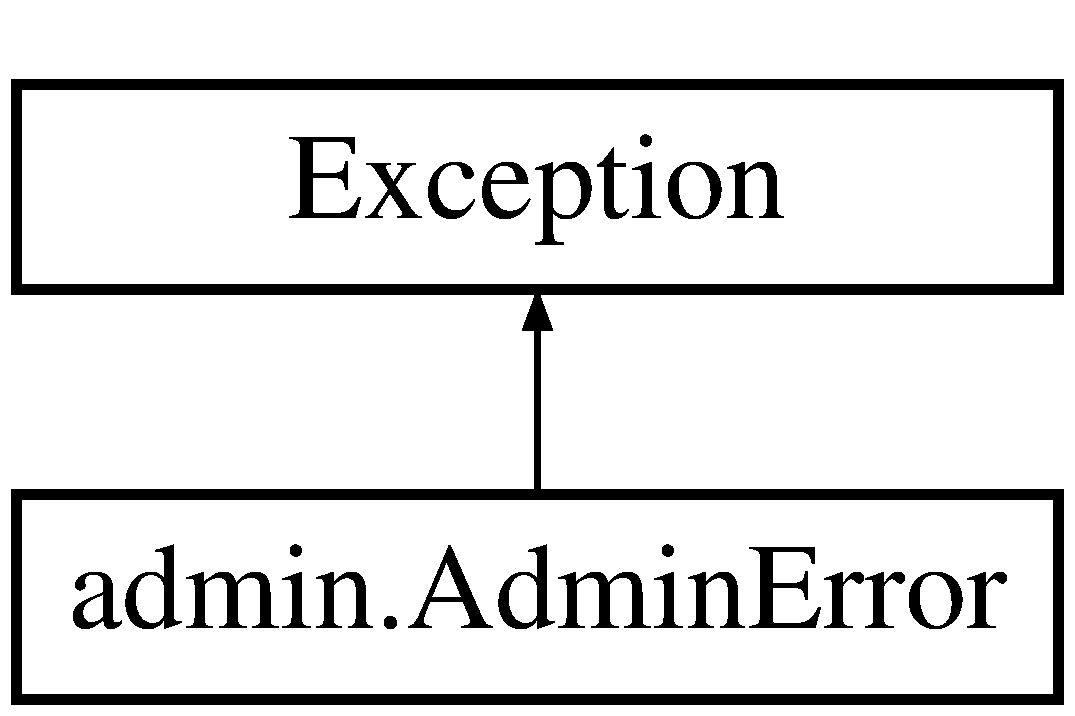
\includegraphics[height=2.000000cm]{df/dee/classadmin_1_1AdminError}
\end{center}
\end{figure}
\subsection*{Public Member Functions}
\begin{DoxyCompactItemize}
\item 
def \hyperlink{classadmin_1_1AdminError_a2712ee3b794fa425e6e0eac6a1524749}{\-\_\-\-\_\-init\-\_\-\-\_\-}
\item 
def \hyperlink{classadmin_1_1AdminError_ab64b4ac0bacc03d3f5d4dc556a493445}{\-\_\-\-\_\-str\-\_\-\-\_\-}
\end{DoxyCompactItemize}
\subsection*{Public Attributes}
\begin{DoxyCompactItemize}
\item 
\hyperlink{classadmin_1_1AdminError_a2d3933c27c7f643bf649f9f208f35c72}{error}
\end{DoxyCompactItemize}


\subsection{Detailed Description}
admin error 

Definition at line 45 of file admin.\-py.



\subsection{Constructor \& Destructor Documentation}
\hypertarget{classadmin_1_1AdminError_a2712ee3b794fa425e6e0eac6a1524749}{\index{admin\-::\-Admin\-Error@{admin\-::\-Admin\-Error}!\-\_\-\-\_\-init\-\_\-\-\_\-@{\-\_\-\-\_\-init\-\_\-\-\_\-}}
\index{\-\_\-\-\_\-init\-\_\-\-\_\-@{\-\_\-\-\_\-init\-\_\-\-\_\-}!admin::AdminError@{admin\-::\-Admin\-Error}}
\subsubsection[{\-\_\-\-\_\-init\-\_\-\-\_\-}]{\setlength{\rightskip}{0pt plus 5cm}def admin.\-Admin\-Error.\-\_\-\-\_\-init\-\_\-\-\_\- (
\begin{DoxyParamCaption}
\item[{}]{self, }
\item[{}]{e}
\end{DoxyParamCaption}
)}}\label{classadmin_1_1AdminError_a2712ee3b794fa425e6e0eac6a1524749}


Definition at line 46 of file admin.\-py.



\subsection{Member Function Documentation}
\hypertarget{classadmin_1_1AdminError_ab64b4ac0bacc03d3f5d4dc556a493445}{\index{admin\-::\-Admin\-Error@{admin\-::\-Admin\-Error}!\-\_\-\-\_\-str\-\_\-\-\_\-@{\-\_\-\-\_\-str\-\_\-\-\_\-}}
\index{\-\_\-\-\_\-str\-\_\-\-\_\-@{\-\_\-\-\_\-str\-\_\-\-\_\-}!admin::AdminError@{admin\-::\-Admin\-Error}}
\subsubsection[{\-\_\-\-\_\-str\-\_\-\-\_\-}]{\setlength{\rightskip}{0pt plus 5cm}def admin.\-Admin\-Error.\-\_\-\-\_\-str\-\_\-\-\_\- (
\begin{DoxyParamCaption}
\item[{}]{self}
\end{DoxyParamCaption}
)}}\label{classadmin_1_1AdminError_ab64b4ac0bacc03d3f5d4dc556a493445}


Definition at line 50 of file admin.\-py.



\subsection{Member Data Documentation}
\hypertarget{classadmin_1_1AdminError_a2d3933c27c7f643bf649f9f208f35c72}{\index{admin\-::\-Admin\-Error@{admin\-::\-Admin\-Error}!error@{error}}
\index{error@{error}!admin::AdminError@{admin\-::\-Admin\-Error}}
\subsubsection[{error}]{\setlength{\rightskip}{0pt plus 5cm}admin.\-Admin\-Error.\-error}}\label{classadmin_1_1AdminError_a2d3933c27c7f643bf649f9f208f35c72}


Definition at line 47 of file admin.\-py.



The documentation for this class was generated from the following file\-:\begin{DoxyCompactItemize}
\item 
\hyperlink{admin_8py}{admin.\-py}\end{DoxyCompactItemize}

\hypertarget{classadmin_1_1build}{\section{admin.\-build Class Reference}
\label{classadmin_1_1build}\index{admin.\-build@{admin.\-build}}
}


Build tools.  


Inheritance diagram for admin.\-build\-:\begin{figure}[H]
\begin{center}
\leavevmode
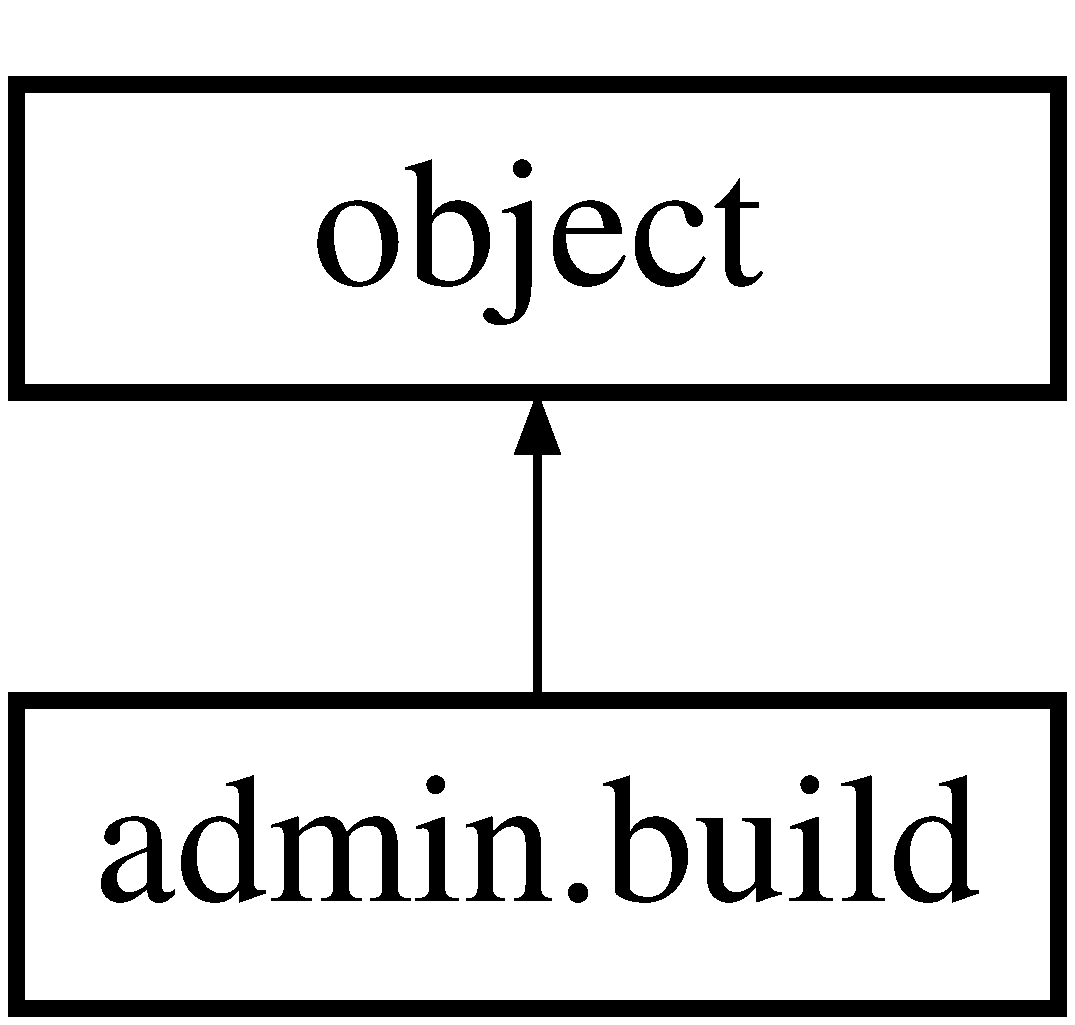
\includegraphics[height=2.000000cm]{d8/dff/classadmin_1_1build}
\end{center}
\end{figure}
\subsection*{Public Member Functions}
\begin{DoxyCompactItemize}
\item 
def \hyperlink{classadmin_1_1build_a265731c57c5b23175db096bf8a76e236}{decode\-\_\-version}
\begin{DoxyCompactList}\small\item\em Decode version information string. \end{DoxyCompactList}\item 
def \hyperlink{classadmin_1_1build_a119269530e1f9f01afc87834d21d722b}{match\-\_\-version}
\begin{DoxyCompactList}\small\item\em Match the specific version. \end{DoxyCompactList}\end{DoxyCompactItemize}
\subsection*{Static Public Member Functions}
\begin{DoxyCompactItemize}
\item 
def \hyperlink{classadmin_1_1build_add65d88734d0ae6b83e8c31cff366b68}{doxygen}
\begin{DoxyCompactList}\small\item\em Generate documentation for codes under Git by Doxygen. \end{DoxyCompactList}\end{DoxyCompactItemize}
\subsection*{Static Public Attributes}
\begin{DoxyCompactItemize}
\item 
tuple \hyperlink{classadmin_1_1build_acf6af7ed40a09ac4e0029edd50a82ae0}{Version} = namedtuple('Version', 'major, minor, patch')
\end{DoxyCompactItemize}


\subsection{Detailed Description}
Build tools. 

This module contains functions and classes for versions, including\-:


\begin{DoxyItemize}
\item Version
\item \hyperlink{classadmin_1_1build_a265731c57c5b23175db096bf8a76e236}{decode\-\_\-version()}, \hyperlink{classadmin_1_1build_a119269530e1f9f01afc87834d21d722b}{match\-\_\-version()} 
\end{DoxyItemize}

Definition at line 266 of file admin.\-py.



\subsection{Member Function Documentation}
\hypertarget{classadmin_1_1build_a265731c57c5b23175db096bf8a76e236}{\index{admin\-::build@{admin\-::build}!decode\-\_\-version@{decode\-\_\-version}}
\index{decode\-\_\-version@{decode\-\_\-version}!admin::build@{admin\-::build}}
\subsubsection[{decode\-\_\-version}]{\setlength{\rightskip}{0pt plus 5cm}def admin.\-build.\-decode\-\_\-version (
\begin{DoxyParamCaption}
\item[{}]{cls, }
\item[{}]{version\-\_\-info, }
\item[{}]{prefix = {\ttfamily ''}}
\end{DoxyParamCaption}
)}}\label{classadmin_1_1build_a265731c57c5b23175db096bf8a76e236}


Decode version information string. 


\begin{DoxyParams}{Parameters}
{\em version\-\_\-info} & version information string (e.\-g. Python 3.\-4.\-1) \\
\hline
{\em prefix} & prefix string of version \\
\hline
\end{DoxyParams}
\begin{DoxyReturn}{Returns}
Version named-\/tuple 
\end{DoxyReturn}


Definition at line 276 of file admin.\-py.

\hypertarget{classadmin_1_1build_add65d88734d0ae6b83e8c31cff366b68}{\index{admin\-::build@{admin\-::build}!doxygen@{doxygen}}
\index{doxygen@{doxygen}!admin::build@{admin\-::build}}
\subsubsection[{doxygen}]{\setlength{\rightskip}{0pt plus 5cm}def admin.\-build.\-doxygen (
\begin{DoxyParamCaption}
\item[{}]{path, }
\item[{}]{doxyfile = {\ttfamily 'Doxyfile.in'}}
\end{DoxyParamCaption}
)\hspace{0.3cm}{\ttfamily [static]}}}\label{classadmin_1_1build_add65d88734d0ae6b83e8c31cff366b68}


Generate documentation for codes under Git by Doxygen. 


\begin{DoxyParams}{Parameters}
{\em path} & project path \\
\hline
{\em doxyfile} & name of Doxygen configuration file \\
\hline
\end{DoxyParams}

\begin{DoxyExceptions}{Exceptions}
{\em subprocess.\-Called\-Process\-Error} & \\
\hline
{\em I\-O\-Error} & \\
\hline
\end{DoxyExceptions}
\begin{DoxySeeAlso}{See Also}
\href{http://www.stack.nl/~dimitri/doxygen/manual/}{\tt http\-://www.\-stack.\-nl/$\sim$dimitri/doxygen/manual/} 
\end{DoxySeeAlso}
\begin{DoxySince}{Since}
Doxygen 1.\-8.\-6 
\end{DoxySince}


Definition at line 318 of file admin.\-py.

\hypertarget{classadmin_1_1build_a119269530e1f9f01afc87834d21d722b}{\index{admin\-::build@{admin\-::build}!match\-\_\-version@{match\-\_\-version}}
\index{match\-\_\-version@{match\-\_\-version}!admin::build@{admin\-::build}}
\subsubsection[{match\-\_\-version}]{\setlength{\rightskip}{0pt plus 5cm}def admin.\-build.\-match\-\_\-version (
\begin{DoxyParamCaption}
\item[{}]{cls, }
\item[{}]{v, }
\item[{}]{match}
\end{DoxyParamCaption}
)}}\label{classadmin_1_1build_a119269530e1f9f01afc87834d21d722b}


Match the specific version. 


\begin{DoxyParams}{Parameters}
{\em v} & Version named-\/tuple \\
\hline
{\em match} & version string (e.\-g. 1.\-2.\-3) \\
\hline
\end{DoxyParams}
\begin{DoxyReturn}{Returns}
True if match 
\end{DoxyReturn}


Definition at line 296 of file admin.\-py.



\subsection{Member Data Documentation}
\hypertarget{classadmin_1_1build_acf6af7ed40a09ac4e0029edd50a82ae0}{\index{admin\-::build@{admin\-::build}!Version@{Version}}
\index{Version@{Version}!admin::build@{admin\-::build}}
\subsubsection[{Version}]{\setlength{\rightskip}{0pt plus 5cm}tuple admin.\-build.\-Version = namedtuple('Version', 'major, minor, patch')\hspace{0.3cm}{\ttfamily [static]}}}\label{classadmin_1_1build_acf6af7ed40a09ac4e0029edd50a82ae0}


Definition at line 268 of file admin.\-py.



The documentation for this class was generated from the following file\-:\begin{DoxyCompactItemize}
\item 
\hyperlink{admin_8py}{admin.\-py}\end{DoxyCompactItemize}

\hypertarget{classadmin_1_1ConfigFile}{\section{admin.\-Config\-File Class Reference}
\label{classadmin_1_1ConfigFile}\index{admin.\-Config\-File@{admin.\-Config\-File}}
}


Configuration file.  


Inheritance diagram for admin.\-Config\-File\-:\begin{figure}[H]
\begin{center}
\leavevmode
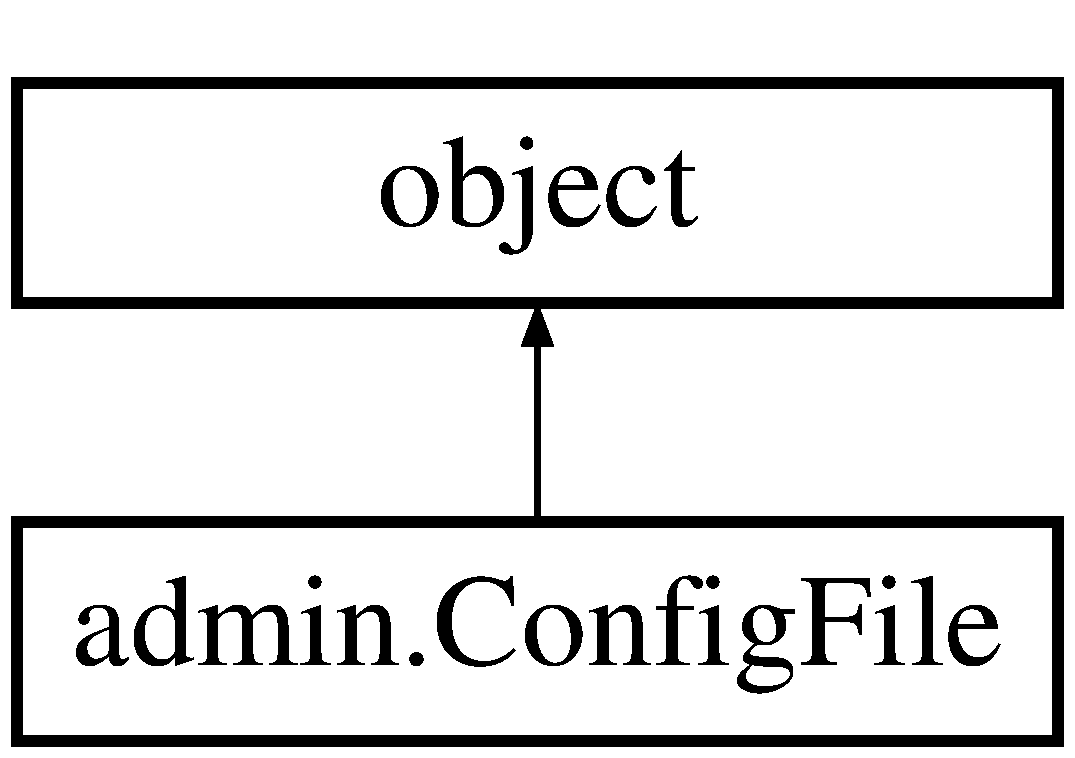
\includegraphics[height=2.000000cm]{d0/d8b/classadmin_1_1ConfigFile}
\end{center}
\end{figure}
\subsection*{Public Member Functions}
\begin{DoxyCompactItemize}
\item 
def \hyperlink{classadmin_1_1ConfigFile_a01f801b702c4cb7e322a8dee7943f5ff}{\-\_\-\-\_\-init\-\_\-\-\_\-}
\begin{DoxyCompactList}\small\item\em Parse configuration file. \end{DoxyCompactList}\item 
def \hyperlink{classadmin_1_1ConfigFile_a3a60d1611c929d782773d73d339454ab}{get}
\begin{DoxyCompactList}\small\item\em Get value of specific option. \end{DoxyCompactList}\item 
def \hyperlink{classadmin_1_1ConfigFile_a05413f3b3760fe95cf8038c400cb2b4f}{set}
\begin{DoxyCompactList}\small\item\em Set value of specific option. \end{DoxyCompactList}\end{DoxyCompactItemize}
\subsection*{Private Attributes}
\begin{DoxyCompactItemize}
\item 
\hyperlink{classadmin_1_1ConfigFile_ada03146a25635d360b9994efcd3eb6ce}{\-\_\-config\-\_\-file}
\item 
\hyperlink{classadmin_1_1ConfigFile_a3f7db562c59049e6a3b28b1fdfafa63e}{\-\_\-sep}
\item 
\hyperlink{classadmin_1_1ConfigFile_ac15829b16933412a7db88d3dacdcf345}{\-\_\-comments}
\item 
\hyperlink{classadmin_1_1ConfigFile_a5a5c415d13ee87e1a03c9f64231a4fc9}{\-\_\-config}
\end{DoxyCompactItemize}


\subsection{Detailed Description}
Configuration file. 

\subsubsection*{Usage}


\begin{DoxyPre}{\ttfamily 
     import os
     import admin}\end{DoxyPre}



\begin{DoxyPre}{\ttfamily      configs = \{'PROJECT\_NAME': '"AAA"',
           'PROJECT\_NUMBER': '1.2.3'\}
     try:
         with open(os.path.join(os.getcwd(), 'Doxyfile'), 'r+') as f:
             config\_file = \hyperlink{classadmin_1_1ConfigFile}{admin.ConfigFile(f)}
             config\_file.set(configs)
         except IOError as e:
             \hyperlink{namespaceadmin_ae1e80d1a965f6551fa95ff379ba2b0cd}{admin.error}('error') 
}\end{DoxyPre}


Definition at line 169 of file \-\_\-\-\_\-init\-\_\-\-\_\-.\-py.



\subsection{Constructor \& Destructor Documentation}
\hypertarget{classadmin_1_1ConfigFile_a01f801b702c4cb7e322a8dee7943f5ff}{\index{admin\-::\-Config\-File@{admin\-::\-Config\-File}!\-\_\-\-\_\-init\-\_\-\-\_\-@{\-\_\-\-\_\-init\-\_\-\-\_\-}}
\index{\-\_\-\-\_\-init\-\_\-\-\_\-@{\-\_\-\-\_\-init\-\_\-\-\_\-}!admin::ConfigFile@{admin\-::\-Config\-File}}
\subsubsection[{\-\_\-\-\_\-init\-\_\-\-\_\-}]{\setlength{\rightskip}{0pt plus 5cm}def admin.\-Config\-File.\-\_\-\-\_\-init\-\_\-\-\_\- (
\begin{DoxyParamCaption}
\item[{}]{self, }
\item[{}]{config\-\_\-file, }
\item[{}]{sep = {\ttfamily '='}, }
\item[{}]{comments = {\ttfamily '\#'}}
\end{DoxyParamCaption}
)}}\label{classadmin_1_1ConfigFile_a01f801b702c4cb7e322a8dee7943f5ff}


Parse configuration file. 


\begin{DoxyParams}{Parameters}
{\em config\-\_\-file} & configuration file object \\
\hline
{\em sep} & separator for option/value pair \\
\hline
{\em comments} & comments leading character \\
\hline
\end{DoxyParams}


Definition at line 175 of file \-\_\-\-\_\-init\-\_\-\-\_\-.\-py.



\subsection{Member Function Documentation}
\hypertarget{classadmin_1_1ConfigFile_a3a60d1611c929d782773d73d339454ab}{\index{admin\-::\-Config\-File@{admin\-::\-Config\-File}!get@{get}}
\index{get@{get}!admin::ConfigFile@{admin\-::\-Config\-File}}
\subsubsection[{get}]{\setlength{\rightskip}{0pt plus 5cm}def admin.\-Config\-File.\-get (
\begin{DoxyParamCaption}
\item[{}]{self, }
\item[{}]{option}
\end{DoxyParamCaption}
)}}\label{classadmin_1_1ConfigFile_a3a60d1611c929d782773d73d339454ab}


Get value of specific option. 


\begin{DoxyParams}{Parameters}
{\em option} & option name \\
\hline
\end{DoxyParams}
\begin{DoxyReturn}{Returns}
option value 
\end{DoxyReturn}

\begin{DoxyExceptions}{Exceptions}
{\em Key\-Error} & -\/ no optinon exists \\
\hline
\end{DoxyExceptions}


Definition at line 195 of file \-\_\-\-\_\-init\-\_\-\-\_\-.\-py.

\hypertarget{classadmin_1_1ConfigFile_a05413f3b3760fe95cf8038c400cb2b4f}{\index{admin\-::\-Config\-File@{admin\-::\-Config\-File}!set@{set}}
\index{set@{set}!admin::ConfigFile@{admin\-::\-Config\-File}}
\subsubsection[{set}]{\setlength{\rightskip}{0pt plus 5cm}def admin.\-Config\-File.\-set (
\begin{DoxyParamCaption}
\item[{}]{self, }
\item[{}]{pairs}
\end{DoxyParamCaption}
)}}\label{classadmin_1_1ConfigFile_a05413f3b3760fe95cf8038c400cb2b4f}


Set value of specific option. 


\begin{DoxyParams}{Parameters}
{\em pairs} & Pairs of option name-\/value. \\
\hline
\end{DoxyParams}


Definition at line 202 of file \-\_\-\-\_\-init\-\_\-\-\_\-.\-py.



\subsection{Member Data Documentation}
\hypertarget{classadmin_1_1ConfigFile_ac15829b16933412a7db88d3dacdcf345}{\index{admin\-::\-Config\-File@{admin\-::\-Config\-File}!\-\_\-comments@{\-\_\-comments}}
\index{\-\_\-comments@{\-\_\-comments}!admin::ConfigFile@{admin\-::\-Config\-File}}
\subsubsection[{\-\_\-comments}]{\setlength{\rightskip}{0pt plus 5cm}admin.\-Config\-File.\-\_\-comments\hspace{0.3cm}{\ttfamily [private]}}}\label{classadmin_1_1ConfigFile_ac15829b16933412a7db88d3dacdcf345}


Definition at line 178 of file \-\_\-\-\_\-init\-\_\-\-\_\-.\-py.

\hypertarget{classadmin_1_1ConfigFile_a5a5c415d13ee87e1a03c9f64231a4fc9}{\index{admin\-::\-Config\-File@{admin\-::\-Config\-File}!\-\_\-config@{\-\_\-config}}
\index{\-\_\-config@{\-\_\-config}!admin::ConfigFile@{admin\-::\-Config\-File}}
\subsubsection[{\-\_\-config}]{\setlength{\rightskip}{0pt plus 5cm}admin.\-Config\-File.\-\_\-config\hspace{0.3cm}{\ttfamily [private]}}}\label{classadmin_1_1ConfigFile_a5a5c415d13ee87e1a03c9f64231a4fc9}


Definition at line 179 of file \-\_\-\-\_\-init\-\_\-\-\_\-.\-py.

\hypertarget{classadmin_1_1ConfigFile_ada03146a25635d360b9994efcd3eb6ce}{\index{admin\-::\-Config\-File@{admin\-::\-Config\-File}!\-\_\-config\-\_\-file@{\-\_\-config\-\_\-file}}
\index{\-\_\-config\-\_\-file@{\-\_\-config\-\_\-file}!admin::ConfigFile@{admin\-::\-Config\-File}}
\subsubsection[{\-\_\-config\-\_\-file}]{\setlength{\rightskip}{0pt plus 5cm}admin.\-Config\-File.\-\_\-config\-\_\-file\hspace{0.3cm}{\ttfamily [private]}}}\label{classadmin_1_1ConfigFile_ada03146a25635d360b9994efcd3eb6ce}


Definition at line 176 of file \-\_\-\-\_\-init\-\_\-\-\_\-.\-py.

\hypertarget{classadmin_1_1ConfigFile_a3f7db562c59049e6a3b28b1fdfafa63e}{\index{admin\-::\-Config\-File@{admin\-::\-Config\-File}!\-\_\-sep@{\-\_\-sep}}
\index{\-\_\-sep@{\-\_\-sep}!admin::ConfigFile@{admin\-::\-Config\-File}}
\subsubsection[{\-\_\-sep}]{\setlength{\rightskip}{0pt plus 5cm}admin.\-Config\-File.\-\_\-sep\hspace{0.3cm}{\ttfamily [private]}}}\label{classadmin_1_1ConfigFile_a3f7db562c59049e6a3b28b1fdfafa63e}


Definition at line 177 of file \-\_\-\-\_\-init\-\_\-\-\_\-.\-py.



The documentation for this class was generated from the following file\-:\begin{DoxyCompactItemize}
\item 
admin/\hyperlink{____init_____8py}{\-\_\-\-\_\-init\-\_\-\-\_\-.\-py}\end{DoxyCompactItemize}

\hypertarget{classadmin_1_1www_1_1nginx}{\section{admin.\-www.\-nginx Class Reference}
\label{classadmin_1_1www_1_1nginx}\index{admin.\-www.\-nginx@{admin.\-www.\-nginx}}
}


nginx server.  


Inheritance diagram for admin.\-www.\-nginx\-:\begin{figure}[H]
\begin{center}
\leavevmode
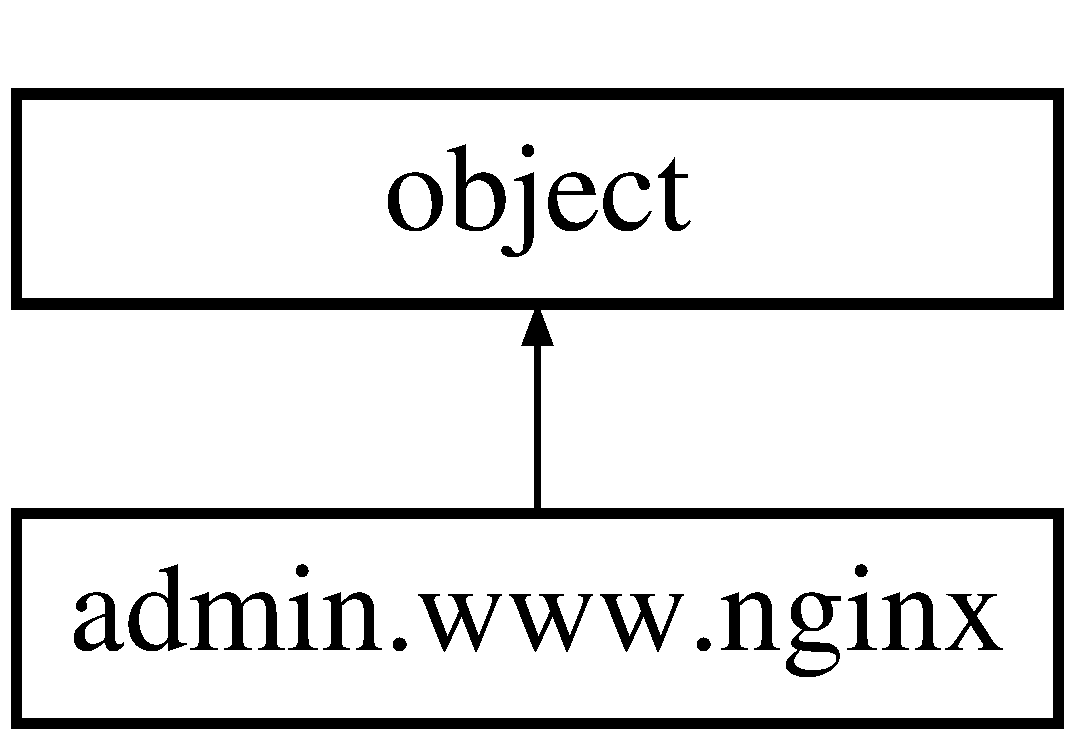
\includegraphics[height=2.000000cm]{dc/db8/classadmin_1_1www_1_1nginx}
\end{center}
\end{figure}
\subsection*{Public Member Functions}
\begin{DoxyCompactItemize}
\item 
def \hyperlink{classadmin_1_1www_1_1nginx_a6d55a9d2645ebdd32a86f07caa30e54f}{enable}
\begin{DoxyCompactList}\small\item\em Setup nginx. \end{DoxyCompactList}\item 
def \hyperlink{classadmin_1_1www_1_1nginx_a97b2603a64e0758b3d548bc1971dcc4e}{disable}
\begin{DoxyCompactList}\small\item\em Disable nginx server. \end{DoxyCompactList}\end{DoxyCompactItemize}
\subsection*{Static Public Attributes}
\begin{DoxyCompactItemize}
\item 
string \hyperlink{classadmin_1_1www_1_1nginx_a0345aad76d9ddd6469c13bef207a9766}{site\-\_\-avail\-\_\-root} = '/etc/\hyperlink{classadmin_1_1www_1_1nginx}{nginx}/sites-\/available'
\item 
string \hyperlink{classadmin_1_1www_1_1nginx_a3e1b0fbd45f31aaeacb6baaec80806ce}{site\-\_\-enable\-\_\-root} = '/etc/\hyperlink{classadmin_1_1www_1_1nginx}{nginx}/sites-\/enabled'
\item 
string \hyperlink{classadmin_1_1www_1_1nginx_aec1e7959ddfe6598718fb6c8c9d72320}{uwsgi\-\_\-params\-\_\-url} = 'https\-://raw.\-githubusercontent.\-com/\hyperlink{classadmin_1_1www_1_1nginx}{nginx}/\hyperlink{classadmin_1_1www_1_1nginx}{nginx}/master/conf/uwsgi\-\_\-params'
\item 
string \hyperlink{classadmin_1_1www_1_1nginx_afd444548cd6faf42c56e24e22148a4b4}{uwsgi\-\_\-params\-\_\-path} = '/etc/\hyperlink{classadmin_1_1www_1_1nginx}{nginx}/uwsgi\-\_\-params'
\end{DoxyCompactItemize}
\subsection*{Private Member Functions}
\begin{DoxyCompactItemize}
\item 
def \hyperlink{classadmin_1_1www_1_1nginx_aca978777776a324a0c3ac506100da002}{\-\_\-site\-\_\-avail\-\_\-path}
\begin{DoxyCompactList}\small\item\em Return path of available site by name. \end{DoxyCompactList}\item 
def \hyperlink{classadmin_1_1www_1_1nginx_af4bc4f7da3d2c56ba8e4b61b16052394}{\-\_\-site\-\_\-enable\-\_\-path}
\begin{DoxyCompactList}\small\item\em Return path of enabled site by name. \end{DoxyCompactList}\end{DoxyCompactItemize}


\subsection{Detailed Description}
nginx server. 

\begin{DoxySeeAlso}{See Also}
\href{http://wiki.nginx.org/Pitfalls}{\tt http\-://wiki.\-nginx.\-org/\-Pitfalls} 

\href{http://wiki.nginx.org/QuickStart}{\tt http\-://wiki.\-nginx.\-org/\-Quick\-Start} 

\href{http://wiki.nginx.org/Configuration}{\tt http\-://wiki.\-nginx.\-org/\-Configuration} 
\end{DoxySeeAlso}
\begin{DoxySince}{Since}
nginx 1.\-4.\-6 
\end{DoxySince}


Definition at line 567 of file admin.\-py.



\subsection{Member Function Documentation}
\hypertarget{classadmin_1_1www_1_1nginx_aca978777776a324a0c3ac506100da002}{\index{admin\-::www\-::nginx@{admin\-::www\-::nginx}!\-\_\-site\-\_\-avail\-\_\-path@{\-\_\-site\-\_\-avail\-\_\-path}}
\index{\-\_\-site\-\_\-avail\-\_\-path@{\-\_\-site\-\_\-avail\-\_\-path}!admin::www::nginx@{admin\-::www\-::nginx}}
\subsubsection[{\-\_\-site\-\_\-avail\-\_\-path}]{\setlength{\rightskip}{0pt plus 5cm}def admin.\-www.\-nginx.\-\_\-site\-\_\-avail\-\_\-path (
\begin{DoxyParamCaption}
\item[{}]{cls, }
\item[{}]{site\-\_\-name}
\end{DoxyParamCaption}
)\hspace{0.3cm}{\ttfamily [private]}}}\label{classadmin_1_1www_1_1nginx_aca978777776a324a0c3ac506100da002}


Return path of available site by name. 


\begin{DoxyParams}{Parameters}
{\em site\-\_\-name} & site name \\
\hline
\end{DoxyParams}
\begin{DoxyReturn}{Returns}
path of given site 
\end{DoxyReturn}


Definition at line 704 of file admin.\-py.

\hypertarget{classadmin_1_1www_1_1nginx_af4bc4f7da3d2c56ba8e4b61b16052394}{\index{admin\-::www\-::nginx@{admin\-::www\-::nginx}!\-\_\-site\-\_\-enable\-\_\-path@{\-\_\-site\-\_\-enable\-\_\-path}}
\index{\-\_\-site\-\_\-enable\-\_\-path@{\-\_\-site\-\_\-enable\-\_\-path}!admin::www::nginx@{admin\-::www\-::nginx}}
\subsubsection[{\-\_\-site\-\_\-enable\-\_\-path}]{\setlength{\rightskip}{0pt plus 5cm}def admin.\-www.\-nginx.\-\_\-site\-\_\-enable\-\_\-path (
\begin{DoxyParamCaption}
\item[{}]{cls, }
\item[{}]{site\-\_\-name = {\ttfamily None}}
\end{DoxyParamCaption}
)\hspace{0.3cm}{\ttfamily [private]}}}\label{classadmin_1_1www_1_1nginx_af4bc4f7da3d2c56ba8e4b61b16052394}


Return path of enabled site by name. 


\begin{DoxyParams}{Parameters}
{\em site\-\_\-name} & site name \\
\hline
\end{DoxyParams}
\begin{DoxyReturn}{Returns}
path of given site 
\end{DoxyReturn}


Definition at line 713 of file admin.\-py.

\hypertarget{classadmin_1_1www_1_1nginx_a97b2603a64e0758b3d548bc1971dcc4e}{\index{admin\-::www\-::nginx@{admin\-::www\-::nginx}!disable@{disable}}
\index{disable@{disable}!admin::www::nginx@{admin\-::www\-::nginx}}
\subsubsection[{disable}]{\setlength{\rightskip}{0pt plus 5cm}def admin.\-www.\-nginx.\-disable (
\begin{DoxyParamCaption}
\item[{}]{cls, }
\item[{}]{site = {\ttfamily None}, }
\item[{}]{upstream = {\ttfamily None}}
\end{DoxyParamCaption}
)}}\label{classadmin_1_1www_1_1nginx_a97b2603a64e0758b3d548bc1971dcc4e}


Disable nginx server. 


\begin{DoxyParams}{Parameters}
{\em site} & site path \\
\hline
{\em upstream} & upstream host address (u\-W\-S\-G\-I gateway) \\
\hline
\end{DoxyParams}

\begin{DoxyExceptions}{Exceptions}
{\em Admin\-Error(subprocess.\-Called\-Process\-Error)} & -\/ shell {\ttfamily sudo ln -\/sf} or {\ttfamily sudo /etc/init.d} error \\
\hline
\end{DoxyExceptions}


Definition at line 688 of file admin.\-py.

\hypertarget{classadmin_1_1www_1_1nginx_a6d55a9d2645ebdd32a86f07caa30e54f}{\index{admin\-::www\-::nginx@{admin\-::www\-::nginx}!enable@{enable}}
\index{enable@{enable}!admin::www::nginx@{admin\-::www\-::nginx}}
\subsubsection[{enable}]{\setlength{\rightskip}{0pt plus 5cm}def admin.\-www.\-nginx.\-enable (
\begin{DoxyParamCaption}
\item[{}]{cls, }
\item[{}]{site, }
\item[{}]{port = {\ttfamily 80}, }
\item[{}]{name = {\ttfamily 'localhost'}, }
\item[{}]{upstream = {\ttfamily None}, }
\item[{}]{proxy = {\ttfamily '\-:8080'}}
\end{DoxyParamCaption}
)}}\label{classadmin_1_1www_1_1nginx_a6d55a9d2645ebdd32a86f07caa30e54f}


Setup nginx. 


\begin{DoxyParams}{Parameters}
{\em site} & site path \\
\hline
{\em port} & site port number \\
\hline
{\em name} & site server name \\
\hline
{\em upstream} & upstream host address (u\-W\-S\-G\-I gateway) \\
\hline
\end{DoxyParams}

\begin{DoxyExceptions}{Exceptions}
{\em I\-O\-Error} & -\/ site configuration file error \\
\hline
{\em Admin\-Error(subprocess.\-Called\-Process\-Error)} & -\/ shell {\ttfamily sudo mv} error \\
\hline
{\em Admin\-Error(subprocess.\-Called\-Process\-Error)} & -\/ download uwsgi\-\_\-params file error \\
\hline
\end{DoxyExceptions}


Definition at line 584 of file admin.\-py.



\subsection{Member Data Documentation}
\hypertarget{classadmin_1_1www_1_1nginx_a0345aad76d9ddd6469c13bef207a9766}{\index{admin\-::www\-::nginx@{admin\-::www\-::nginx}!site\-\_\-avail\-\_\-root@{site\-\_\-avail\-\_\-root}}
\index{site\-\_\-avail\-\_\-root@{site\-\_\-avail\-\_\-root}!admin::www::nginx@{admin\-::www\-::nginx}}
\subsubsection[{site\-\_\-avail\-\_\-root}]{\setlength{\rightskip}{0pt plus 5cm}string admin.\-www.\-nginx.\-site\-\_\-avail\-\_\-root = '/etc/{\bf nginx}/sites-\/available'\hspace{0.3cm}{\ttfamily [static]}}}\label{classadmin_1_1www_1_1nginx_a0345aad76d9ddd6469c13bef207a9766}


Definition at line 569 of file admin.\-py.

\hypertarget{classadmin_1_1www_1_1nginx_a3e1b0fbd45f31aaeacb6baaec80806ce}{\index{admin\-::www\-::nginx@{admin\-::www\-::nginx}!site\-\_\-enable\-\_\-root@{site\-\_\-enable\-\_\-root}}
\index{site\-\_\-enable\-\_\-root@{site\-\_\-enable\-\_\-root}!admin::www::nginx@{admin\-::www\-::nginx}}
\subsubsection[{site\-\_\-enable\-\_\-root}]{\setlength{\rightskip}{0pt plus 5cm}string admin.\-www.\-nginx.\-site\-\_\-enable\-\_\-root = '/etc/{\bf nginx}/sites-\/enabled'\hspace{0.3cm}{\ttfamily [static]}}}\label{classadmin_1_1www_1_1nginx_a3e1b0fbd45f31aaeacb6baaec80806ce}


Definition at line 570 of file admin.\-py.

\hypertarget{classadmin_1_1www_1_1nginx_afd444548cd6faf42c56e24e22148a4b4}{\index{admin\-::www\-::nginx@{admin\-::www\-::nginx}!uwsgi\-\_\-params\-\_\-path@{uwsgi\-\_\-params\-\_\-path}}
\index{uwsgi\-\_\-params\-\_\-path@{uwsgi\-\_\-params\-\_\-path}!admin::www::nginx@{admin\-::www\-::nginx}}
\subsubsection[{uwsgi\-\_\-params\-\_\-path}]{\setlength{\rightskip}{0pt plus 5cm}string admin.\-www.\-nginx.\-uwsgi\-\_\-params\-\_\-path = '/etc/{\bf nginx}/uwsgi\-\_\-params'\hspace{0.3cm}{\ttfamily [static]}}}\label{classadmin_1_1www_1_1nginx_afd444548cd6faf42c56e24e22148a4b4}


Definition at line 572 of file admin.\-py.

\hypertarget{classadmin_1_1www_1_1nginx_aec1e7959ddfe6598718fb6c8c9d72320}{\index{admin\-::www\-::nginx@{admin\-::www\-::nginx}!uwsgi\-\_\-params\-\_\-url@{uwsgi\-\_\-params\-\_\-url}}
\index{uwsgi\-\_\-params\-\_\-url@{uwsgi\-\_\-params\-\_\-url}!admin::www::nginx@{admin\-::www\-::nginx}}
\subsubsection[{uwsgi\-\_\-params\-\_\-url}]{\setlength{\rightskip}{0pt plus 5cm}string admin.\-www.\-nginx.\-uwsgi\-\_\-params\-\_\-url = 'https\-://raw.\-githubusercontent.\-com/{\bf nginx}/{\bf nginx}/master/conf/uwsgi\-\_\-params'\hspace{0.3cm}{\ttfamily [static]}}}\label{classadmin_1_1www_1_1nginx_aec1e7959ddfe6598718fb6c8c9d72320}


Definition at line 571 of file admin.\-py.



The documentation for this class was generated from the following file\-:\begin{DoxyCompactItemize}
\item 
\hyperlink{admin_8py}{admin.\-py}\end{DoxyCompactItemize}

\hypertarget{classadmin_1_1shell}{\section{admin.\-shell Class Reference}
\label{classadmin_1_1shell}\index{admin.\-shell@{admin.\-shell}}
}


Linux shell tools.  


Inheritance diagram for admin.\-shell\-:\begin{figure}[H]
\begin{center}
\leavevmode
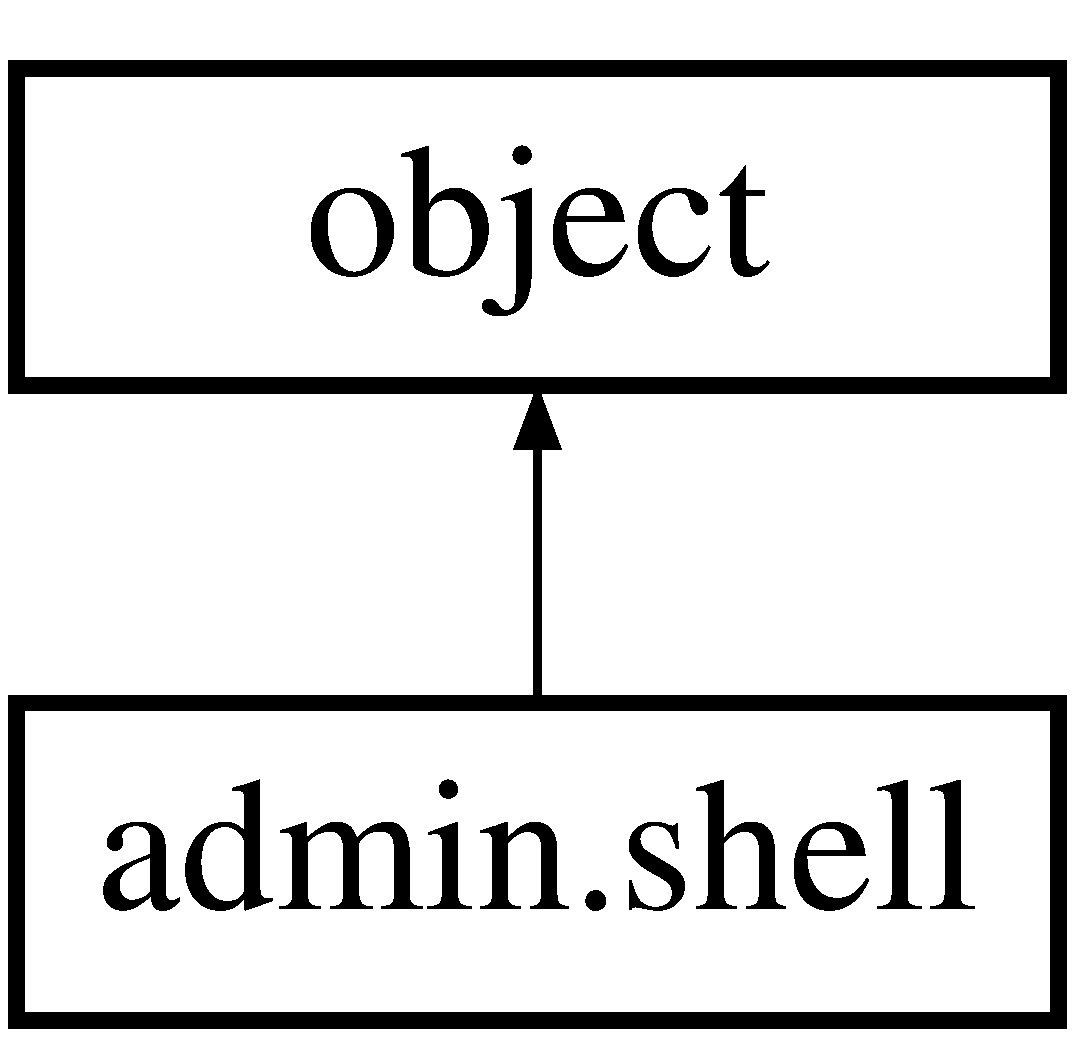
\includegraphics[height=2.000000cm]{de/d16/classadmin_1_1shell}
\end{center}
\end{figure}
\subsection*{Public Member Functions}
\begin{DoxyCompactItemize}
\item 
def \hyperlink{classadmin_1_1shell_a539012368a068a40cd347acbe49989d5}{chown}
\begin{DoxyCompactList}\small\item\em Change owner user and group of the given path. \end{DoxyCompactList}\item 
def \hyperlink{classadmin_1_1shell_ad4f8d9280283a993eec0bc5dcade6d99}{remove}
\begin{DoxyCompactList}\small\item\em Remove path entry. \end{DoxyCompactList}\item 
def \hyperlink{classadmin_1_1shell_adcdf00aa6acc1cf519ece418ce14a7f1}{mkdir}
\begin{DoxyCompactList}\small\item\em Create a directory or directories recursively. \end{DoxyCompactList}\item 
def \hyperlink{classadmin_1_1shell_a9cc97c2976b95fbcfa88b314803aa2bf}{symlink}
\begin{DoxyCompactList}\small\item\em Create a symbolic link pointing to source named {\ttfamily link\-\_\-name}. \end{DoxyCompactList}\item 
def \hyperlink{classadmin_1_1shell_a432e79bf26b0adb3e7fcf2f13f96229e}{start\-\_\-init\-\_\-service}
\begin{DoxyCompactList}\small\item\em Start init service. \end{DoxyCompactList}\item 
def \hyperlink{classadmin_1_1shell_a20ba085e92f2f4a9332d8d9c95ce7aa1}{stop\-\_\-init\-\_\-service}
\begin{DoxyCompactList}\small\item\em Stop init service. \end{DoxyCompactList}\item 
def \hyperlink{classadmin_1_1shell_ab6f38a2fae6ea2cc870c1de2d6cb6017}{restart\-\_\-init\-\_\-service}
\begin{DoxyCompactList}\small\item\em Restart init service. \end{DoxyCompactList}\end{DoxyCompactItemize}
\subsection*{Static Public Member Functions}
\begin{DoxyCompactItemize}
\item 
def \hyperlink{classadmin_1_1shell_a2ffff5c7d8eb2d2cc174df10ac1523b2}{shell}
\begin{DoxyCompactList}\small\item\em Run shell command without output. \end{DoxyCompactList}\item 
def \hyperlink{classadmin_1_1shell_a088a4609cf54f76ee4c838eea157fbc9}{read\-\_\-lines}
\begin{DoxyCompactList}\small\item\em Read specific line(s) with line number(s). \end{DoxyCompactList}\item 
def \hyperlink{classadmin_1_1shell_a5200a0188543eaaa2eb33fc295da0733}{eintr\-\_\-retry}
\begin{DoxyCompactList}\small\item\em Restart a system call interrupted by {\ttfamily E\-I\-N\-T\-R}. \end{DoxyCompactList}\item 
def \hyperlink{classadmin_1_1shell_a79f2a3efc85b54c29621697087299778}{cpu\-\_\-cores}
\end{DoxyCompactItemize}


\subsection{Detailed Description}
Linux shell tools. 

This module contains functions and classes for Linux shell, including\-:


\begin{DoxyItemize}
\item \hyperlink{classadmin_1_1shell_a2ffff5c7d8eb2d2cc174df10ac1523b2}{shell()}, \hyperlink{classadmin_1_1shell_a539012368a068a40cd347acbe49989d5}{chown()}, \hyperlink{classadmin_1_1shell_ad4f8d9280283a993eec0bc5dcade6d99}{remove()}, \hyperlink{classadmin_1_1shell_adcdf00aa6acc1cf519ece418ce14a7f1}{mkdir()}, \hyperlink{classadmin_1_1shell_a9cc97c2976b95fbcfa88b314803aa2bf}{symlink()}
\item \hyperlink{classadmin_1_1shell_a432e79bf26b0adb3e7fcf2f13f96229e}{start\-\_\-init\-\_\-service()}, \hyperlink{classadmin_1_1shell_a20ba085e92f2f4a9332d8d9c95ce7aa1}{stop\-\_\-init\-\_\-service()}, \hyperlink{classadmin_1_1shell_ab6f38a2fae6ea2cc870c1de2d6cb6017}{restart\-\_\-init\-\_\-service()}
\item \hyperlink{classadmin_1_1shell_a088a4609cf54f76ee4c838eea157fbc9}{read\-\_\-lines()}
\item \hyperlink{classadmin_1_1shell_a5200a0188543eaaa2eb33fc295da0733}{eintr\-\_\-retry()}
\item \hyperlink{classadmin_1_1shell_a79f2a3efc85b54c29621697087299778}{cpu\-\_\-cores()} (Only /proc supported system) 
\end{DoxyItemize}

Definition at line 71 of file admin.\-py.



\subsection{Constructor \& Destructor Documentation}
\hypertarget{classadmin_1_1shell_a2ffff5c7d8eb2d2cc174df10ac1523b2}{\index{admin\-::shell@{admin\-::shell}!shell@{shell}}
\index{shell@{shell}!admin::shell@{admin\-::shell}}
\subsubsection[{shell}]{\setlength{\rightskip}{0pt plus 5cm}def admin.\-shell.\-shell (
\begin{DoxyParamCaption}
\item[{}]{cmd}
\end{DoxyParamCaption}
)\hspace{0.3cm}{\ttfamily [static]}}}\label{classadmin_1_1shell_a2ffff5c7d8eb2d2cc174df10ac1523b2}


Run shell command without output. 


\begin{DoxyParams}{Parameters}
{\em cmd} & shell command \\
\hline
\end{DoxyParams}

\begin{DoxyExceptions}{Exceptions}
{\em Admin\-Error(subprocess.\-Called\-Process\-Error)} & -\/ shell command error \\
\hline
\end{DoxyExceptions}


Definition at line 78 of file admin.\-py.



\subsection{Member Function Documentation}
\hypertarget{classadmin_1_1shell_a539012368a068a40cd347acbe49989d5}{\index{admin\-::shell@{admin\-::shell}!chown@{chown}}
\index{chown@{chown}!admin::shell@{admin\-::shell}}
\subsubsection[{chown}]{\setlength{\rightskip}{0pt plus 5cm}def admin.\-shell.\-chown (
\begin{DoxyParamCaption}
\item[{}]{cls, }
\item[{}]{path, }
\item[{}]{user, }
\item[{}]{group = {\ttfamily None}}
\end{DoxyParamCaption}
)}}\label{classadmin_1_1shell_a539012368a068a40cd347acbe49989d5}


Change owner user and group of the given path. 


\begin{DoxyParams}{Parameters}
{\em path} & path whose ownership to be changed \\
\hline
{\em user} & owner user name or uid \\
\hline
{\em group} & owner group name or gid \\
\hline
\end{DoxyParams}

\begin{DoxyExceptions}{Exceptions}
{\em Admin\-Error(\-Value\-Error)} & -\/ both user or group not given \\
\hline
{\em Admin\-Error(\-Lookup\-Error)} & -\/ user or group given not in system \\
\hline
{\em Admin\-Error(subprocess.\-Called\-Process\-Error)} & -\/ shell {\ttfamily sudo chown} error \\
\hline
\end{DoxyExceptions}


Definition at line 94 of file admin.\-py.

\hypertarget{classadmin_1_1shell_a79f2a3efc85b54c29621697087299778}{\index{admin\-::shell@{admin\-::shell}!cpu\-\_\-cores@{cpu\-\_\-cores}}
\index{cpu\-\_\-cores@{cpu\-\_\-cores}!admin::shell@{admin\-::shell}}
\subsubsection[{cpu\-\_\-cores}]{\setlength{\rightskip}{0pt plus 5cm}def admin.\-shell.\-cpu\-\_\-cores (
\begin{DoxyParamCaption}
{}
\end{DoxyParamCaption}
)\hspace{0.3cm}{\ttfamily [static]}}}\label{classadmin_1_1shell_a79f2a3efc85b54c29621697087299778}


Definition at line 252 of file admin.\-py.

\hypertarget{classadmin_1_1shell_a5200a0188543eaaa2eb33fc295da0733}{\index{admin\-::shell@{admin\-::shell}!eintr\-\_\-retry@{eintr\-\_\-retry}}
\index{eintr\-\_\-retry@{eintr\-\_\-retry}!admin::shell@{admin\-::shell}}
\subsubsection[{eintr\-\_\-retry}]{\setlength{\rightskip}{0pt plus 5cm}def admin.\-shell.\-eintr\-\_\-retry (
\begin{DoxyParamCaption}
\item[{}]{func, }
\item[{}]{args}
\end{DoxyParamCaption}
)\hspace{0.3cm}{\ttfamily [static]}}}\label{classadmin_1_1shell_a5200a0188543eaaa2eb33fc295da0733}


Restart a system call interrupted by {\ttfamily E\-I\-N\-T\-R}. 


\begin{DoxyParams}{Parameters}
{\em func} & system call \\
\hline
{\em args} & arguments of system call \\
\hline
\end{DoxyParams}

\begin{DoxyExceptions}{Exceptions}
{\em socket.\-error} & -\/ socket error \\
\hline
{\em select.\-error} & -\/ select module error \\
\hline
{\em O\-S\-Error} & -\/ other O\-S errors \\
\hline
\end{DoxyExceptions}


Definition at line 238 of file admin.\-py.

\hypertarget{classadmin_1_1shell_adcdf00aa6acc1cf519ece418ce14a7f1}{\index{admin\-::shell@{admin\-::shell}!mkdir@{mkdir}}
\index{mkdir@{mkdir}!admin::shell@{admin\-::shell}}
\subsubsection[{mkdir}]{\setlength{\rightskip}{0pt plus 5cm}def admin.\-shell.\-mkdir (
\begin{DoxyParamCaption}
\item[{}]{cls, }
\item[{}]{path, }
\item[{}]{user = {\ttfamily None}, }
\item[{}]{group = {\ttfamily None}}
\end{DoxyParamCaption}
)}}\label{classadmin_1_1shell_adcdf00aa6acc1cf519ece418ce14a7f1}


Create a directory or directories recursively. 


\begin{DoxyParams}{Parameters}
{\em path} & directory path \\
\hline
{\em user} & owner user name or uid \\
\hline
{\em group} & owner group name or gid \\
\hline
\end{DoxyParams}

\begin{DoxyExceptions}{Exceptions}
{\em Admin\-Error(subprocess.\-Called\-Process\-Error)} & -\/ shell {\ttfamily sudo mkdir} error \\
\hline
{\em Admin\-Error(\-Value\-Error)} & -\/ both user or group not given \\
\hline
{\em Admin\-Error(\-Lookup\-Error)} & -\/ user or group given not in system \\
\hline
{\em Admin\-Error(subprocess.\-Called\-Process\-Error)} & -\/ change ownership error\\
\hline
\end{DoxyExceptions}
\begin{DoxySince}{Since}
Python 3.\-2 
\end{DoxySince}


Definition at line 156 of file admin.\-py.

\hypertarget{classadmin_1_1shell_a088a4609cf54f76ee4c838eea157fbc9}{\index{admin\-::shell@{admin\-::shell}!read\-\_\-lines@{read\-\_\-lines}}
\index{read\-\_\-lines@{read\-\_\-lines}!admin::shell@{admin\-::shell}}
\subsubsection[{read\-\_\-lines}]{\setlength{\rightskip}{0pt plus 5cm}def admin.\-shell.\-read\-\_\-lines (
\begin{DoxyParamCaption}
\item[{}]{filename, }
\item[{}]{lineno}
\end{DoxyParamCaption}
)\hspace{0.3cm}{\ttfamily [static]}}}\label{classadmin_1_1shell_a088a4609cf54f76ee4c838eea157fbc9}


Read specific line(s) with line number(s). 


\begin{DoxyParams}{Parameters}
{\em filename} & file name \\
\hline
{\em lineno} & line number(s) to read (starting with 1) \\
\hline
\end{DoxyParams}
\begin{DoxyReturn}{Returns}
generator object of line with no terminating line break 
\end{DoxyReturn}

\begin{DoxyExceptions}{Exceptions}
{\em Type\-Error,I\-O\-Error} & \\
\hline
\end{DoxyExceptions}


Definition at line 217 of file admin.\-py.

\hypertarget{classadmin_1_1shell_ad4f8d9280283a993eec0bc5dcade6d99}{\index{admin\-::shell@{admin\-::shell}!remove@{remove}}
\index{remove@{remove}!admin::shell@{admin\-::shell}}
\subsubsection[{remove}]{\setlength{\rightskip}{0pt plus 5cm}def admin.\-shell.\-remove (
\begin{DoxyParamCaption}
\item[{}]{cls, }
\item[{}]{path}
\end{DoxyParamCaption}
)}}\label{classadmin_1_1shell_ad4f8d9280283a993eec0bc5dcade6d99}


Remove path entry. 


\begin{DoxyParams}{Parameters}
{\em path} & path name of entry to be removed \\
\hline
\end{DoxyParams}

\begin{DoxyExceptions}{Exceptions}
{\em Admin\-Error(subprocess.\-Called\-Process\-Error)} & -\/ shell 'sudo rm -\/f' error \\
\hline
\end{DoxyExceptions}


Definition at line 125 of file admin.\-py.

\hypertarget{classadmin_1_1shell_ab6f38a2fae6ea2cc870c1de2d6cb6017}{\index{admin\-::shell@{admin\-::shell}!restart\-\_\-init\-\_\-service@{restart\-\_\-init\-\_\-service}}
\index{restart\-\_\-init\-\_\-service@{restart\-\_\-init\-\_\-service}!admin::shell@{admin\-::shell}}
\subsubsection[{restart\-\_\-init\-\_\-service}]{\setlength{\rightskip}{0pt plus 5cm}def admin.\-shell.\-restart\-\_\-init\-\_\-service (
\begin{DoxyParamCaption}
\item[{}]{cls, }
\item[{}]{service}
\end{DoxyParamCaption}
)}}\label{classadmin_1_1shell_ab6f38a2fae6ea2cc870c1de2d6cb6017}


Restart init service. 


\begin{DoxyParams}{Parameters}
{\em service} & service name \\
\hline
\end{DoxyParams}

\begin{DoxyExceptions}{Exceptions}
{\em Admin\-Error(subprocess.\-Called\-Process\-Error)} & -\/ shell {\ttfamily sudo /etc/init.d} error \\
\hline
\end{DoxyExceptions}


Definition at line 206 of file admin.\-py.

\hypertarget{classadmin_1_1shell_a432e79bf26b0adb3e7fcf2f13f96229e}{\index{admin\-::shell@{admin\-::shell}!start\-\_\-init\-\_\-service@{start\-\_\-init\-\_\-service}}
\index{start\-\_\-init\-\_\-service@{start\-\_\-init\-\_\-service}!admin::shell@{admin\-::shell}}
\subsubsection[{start\-\_\-init\-\_\-service}]{\setlength{\rightskip}{0pt plus 5cm}def admin.\-shell.\-start\-\_\-init\-\_\-service (
\begin{DoxyParamCaption}
\item[{}]{cls, }
\item[{}]{service}
\end{DoxyParamCaption}
)}}\label{classadmin_1_1shell_a432e79bf26b0adb3e7fcf2f13f96229e}


Start init service. 


\begin{DoxyParams}{Parameters}
{\em service} & service name \\
\hline
\end{DoxyParams}

\begin{DoxyExceptions}{Exceptions}
{\em Admin\-Error(subprocess.\-Called\-Process\-Error)} & -\/ shell {\ttfamily sudo /etc/init.d} error \\
\hline
\end{DoxyExceptions}


Definition at line 188 of file admin.\-py.

\hypertarget{classadmin_1_1shell_a20ba085e92f2f4a9332d8d9c95ce7aa1}{\index{admin\-::shell@{admin\-::shell}!stop\-\_\-init\-\_\-service@{stop\-\_\-init\-\_\-service}}
\index{stop\-\_\-init\-\_\-service@{stop\-\_\-init\-\_\-service}!admin::shell@{admin\-::shell}}
\subsubsection[{stop\-\_\-init\-\_\-service}]{\setlength{\rightskip}{0pt plus 5cm}def admin.\-shell.\-stop\-\_\-init\-\_\-service (
\begin{DoxyParamCaption}
\item[{}]{cls, }
\item[{}]{service}
\end{DoxyParamCaption}
)}}\label{classadmin_1_1shell_a20ba085e92f2f4a9332d8d9c95ce7aa1}


Stop init service. 


\begin{DoxyParams}{Parameters}
{\em service} & service name \\
\hline
\end{DoxyParams}

\begin{DoxyExceptions}{Exceptions}
{\em Admin\-Error(subprocess.\-Called\-Process\-Error)} & -\/ shell {\ttfamily sudo /etc/init.d} error \\
\hline
\end{DoxyExceptions}


Definition at line 197 of file admin.\-py.

\hypertarget{classadmin_1_1shell_a9cc97c2976b95fbcfa88b314803aa2bf}{\index{admin\-::shell@{admin\-::shell}!symlink@{symlink}}
\index{symlink@{symlink}!admin::shell@{admin\-::shell}}
\subsubsection[{symlink}]{\setlength{\rightskip}{0pt plus 5cm}def admin.\-shell.\-symlink (
\begin{DoxyParamCaption}
\item[{}]{cls, }
\item[{}]{src, }
\item[{}]{link\-\_\-name}
\end{DoxyParamCaption}
)}}\label{classadmin_1_1shell_a9cc97c2976b95fbcfa88b314803aa2bf}


Create a symbolic link pointing to source named {\ttfamily link\-\_\-name}. 


\begin{DoxyParams}{Parameters}
{\em src} & source file \\
\hline
{\em link\-\_\-name} & symbolic link name \\
\hline
\end{DoxyParams}

\begin{DoxyExceptions}{Exceptions}
{\em Admin\-Error(subprocess.\-Called\-Process\-Error)} & -\/ shell {\ttfamily sudo ln -\/sf} error \\
\hline
\end{DoxyExceptions}


Definition at line 173 of file admin.\-py.



The documentation for this class was generated from the following file\-:\begin{DoxyCompactItemize}
\item 
\hyperlink{admin_8py}{admin.\-py}\end{DoxyCompactItemize}

\hypertarget{classadmin_1_1www_1_1uwsgi}{\section{admin.\-www.\-uwsgi Class Reference}
\label{classadmin_1_1www_1_1uwsgi}\index{admin.\-www.\-uwsgi@{admin.\-www.\-uwsgi}}
}


u\-W\-S\-G\-I server.  


Inheritance diagram for admin.\-www.\-uwsgi\-:\begin{figure}[H]
\begin{center}
\leavevmode
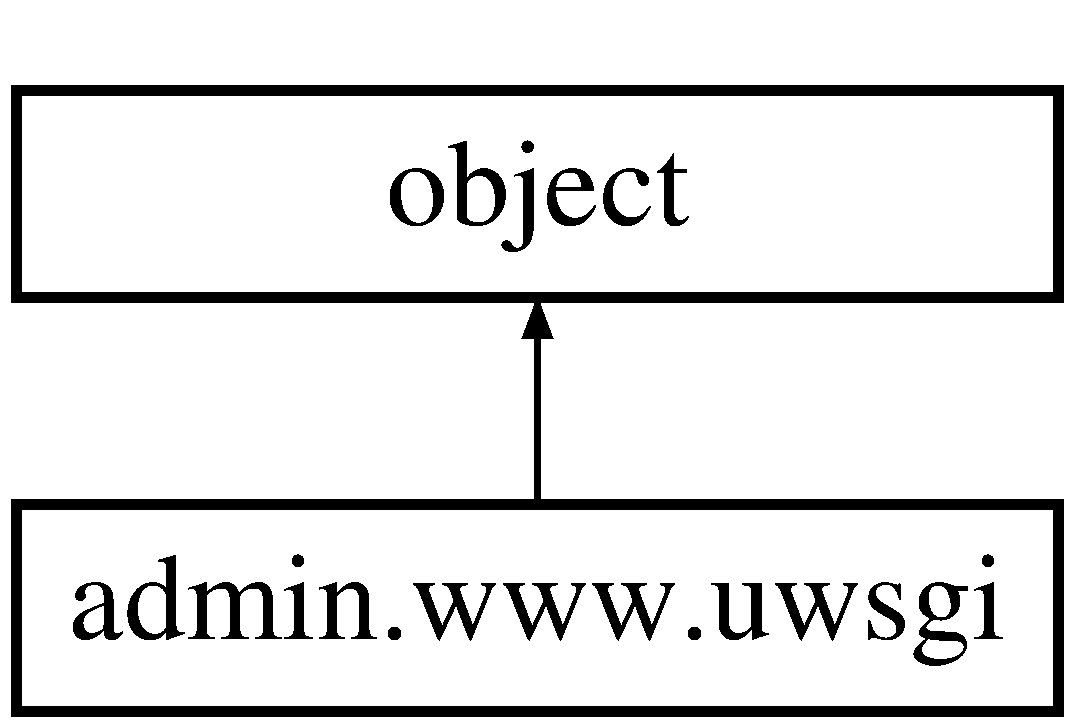
\includegraphics[height=2.000000cm]{db/de4/classadmin_1_1www_1_1uwsgi}
\end{center}
\end{figure}
\subsection*{Public Member Functions}
\begin{DoxyCompactItemize}
\item 
def \hyperlink{classadmin_1_1www_1_1uwsgi_ab5860b95c90e736ad96fb7273efa10a5}{run}
\begin{DoxyCompactList}\small\item\em Run (or Reload) u\-W\-S\-G\-I server. \end{DoxyCompactList}\item 
def \hyperlink{classadmin_1_1www_1_1uwsgi_a01b2b5c841e2da98a5e88286de95bd05}{stop}
\begin{DoxyCompactList}\small\item\em Stop u\-W\-S\-G\-I server. \end{DoxyCompactList}\end{DoxyCompactItemize}
\subsection*{Static Private Member Functions}
\begin{DoxyCompactItemize}
\item 
def \hyperlink{classadmin_1_1www_1_1uwsgi_aefa1ab9824e26e8da07141806cd69ed7}{\-\_\-pidfile}
\begin{DoxyCompactList}\small\item\em Return u\-W\-S\-G\-I pid file from app name. \end{DoxyCompactList}\end{DoxyCompactItemize}


\subsection{Detailed Description}
u\-W\-S\-G\-I server. 

\begin{DoxySeeAlso}{See Also}
\href{https://uwsgi.readthedocs.org/en/latest/index.html}{\tt https\-://uwsgi.\-readthedocs.\-org/en/latest/index.\-html} 
\end{DoxySeeAlso}
\begin{DoxySince}{Since}
u\-W\-S\-G\-I 2.\-0.\-6 
\end{DoxySince}


Definition at line 436 of file admin.\-py.



\subsection{Member Function Documentation}
\hypertarget{classadmin_1_1www_1_1uwsgi_aefa1ab9824e26e8da07141806cd69ed7}{\index{admin\-::www\-::uwsgi@{admin\-::www\-::uwsgi}!\-\_\-pidfile@{\-\_\-pidfile}}
\index{\-\_\-pidfile@{\-\_\-pidfile}!admin::www::uwsgi@{admin\-::www\-::uwsgi}}
\subsubsection[{\-\_\-pidfile}]{\setlength{\rightskip}{0pt plus 5cm}def admin.\-www.\-uwsgi.\-\_\-pidfile (
\begin{DoxyParamCaption}
\item[{}]{app}
\end{DoxyParamCaption}
)\hspace{0.3cm}{\ttfamily [static]}, {\ttfamily [private]}}}\label{classadmin_1_1www_1_1uwsgi_aefa1ab9824e26e8da07141806cd69ed7}


Return u\-W\-S\-G\-I pid file from app name. 


\begin{DoxyParams}{Parameters}
{\em app} & app name \\
\hline
\end{DoxyParams}


Definition at line 557 of file admin.\-py.

\hypertarget{classadmin_1_1www_1_1uwsgi_ab5860b95c90e736ad96fb7273efa10a5}{\index{admin\-::www\-::uwsgi@{admin\-::www\-::uwsgi}!run@{run}}
\index{run@{run}!admin::www::uwsgi@{admin\-::www\-::uwsgi}}
\subsubsection[{run}]{\setlength{\rightskip}{0pt plus 5cm}def admin.\-www.\-uwsgi.\-run (
\begin{DoxyParamCaption}
\item[{}]{cls, }
\item[{}]{app, }
\item[{}]{addr, }
\item[{}]{init = {\ttfamily False}, }
\item[{}]{gateway = {\ttfamily False}}
\end{DoxyParamCaption}
)}}\label{classadmin_1_1www_1_1uwsgi_ab5860b95c90e736ad96fb7273efa10a5}


Run (or Reload) u\-W\-S\-G\-I server. 


\begin{DoxyParams}{Parameters}
{\em app} & app (absolute) path \\
\hline
{\em addr} & u\-W\-S\-G\-I server address \\
\hline
{\em init} & True for adding to init system \\
\hline
{\em gateway} & True for internal gateway \\
\hline
\end{DoxyParams}

\begin{DoxyExceptions}{Exceptions}
{\em Value\-Error} & -\/ app path not absolute path \\
\hline
{\em Admin\-Error(subprocess.\-Called\-Process\-Error)} & -\/ shell error \\
\hline
{\em I\-O\-Error} & -\/ configuration file error\\
\hline
\end{DoxyExceptions}
N\-O\-T\-E\-: Before run u\-W\-S\-G\-I with Django, make sure that Django project actually works\-: \begin{DoxyVerb}python manage.py runserver 0.0.0.0:8000
\end{DoxyVerb}


\begin{DoxySeeAlso}{See Also}
\href{https://www.djangoproject.com/}{\tt https\-://www.\-djangoproject.\-com/} 
\end{DoxySeeAlso}
\begin{DoxySince}{Since}
Django 1.\-7 

Python 3.\-2 
\end{DoxySince}


Definition at line 457 of file admin.\-py.

\hypertarget{classadmin_1_1www_1_1uwsgi_a01b2b5c841e2da98a5e88286de95bd05}{\index{admin\-::www\-::uwsgi@{admin\-::www\-::uwsgi}!stop@{stop}}
\index{stop@{stop}!admin::www::uwsgi@{admin\-::www\-::uwsgi}}
\subsubsection[{stop}]{\setlength{\rightskip}{0pt plus 5cm}def admin.\-www.\-uwsgi.\-stop (
\begin{DoxyParamCaption}
\item[{}]{cls, }
\item[{}]{app}
\end{DoxyParamCaption}
)}}\label{classadmin_1_1www_1_1uwsgi_a01b2b5c841e2da98a5e88286de95bd05}


Stop u\-W\-S\-G\-I server. 


\begin{DoxyParams}{Parameters}
{\em app} & app (absolute) path \\
\hline
\end{DoxyParams}

\begin{DoxyExceptions}{Exceptions}
{\em Admin\-Error(subprocess.\-Called\-Process\-Error)} & -\/ shell error \\
\hline
\end{DoxyExceptions}


Definition at line 546 of file admin.\-py.



The documentation for this class was generated from the following file\-:\begin{DoxyCompactItemize}
\item 
\hyperlink{admin_8py}{admin.\-py}\end{DoxyCompactItemize}

\hypertarget{classadmin_1_1www}{\section{admin.\-www Class Reference}
\label{classadmin_1_1www}\index{admin.\-www@{admin.\-www}}
}


W\-W\-W (Internet) tools.  


Inheritance diagram for admin.\-www\-:\begin{figure}[H]
\begin{center}
\leavevmode
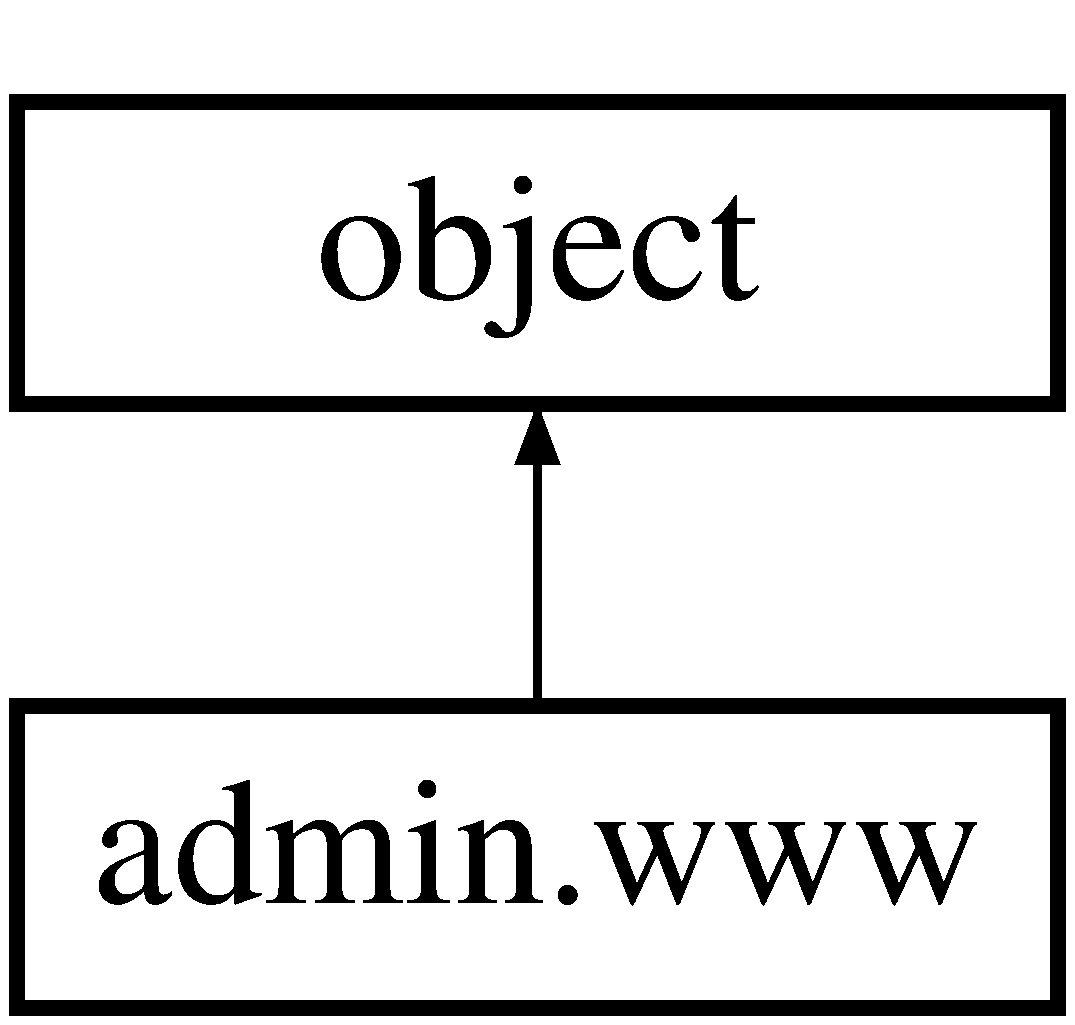
\includegraphics[height=2.000000cm]{d6/dae/classadmin_1_1www}
\end{center}
\end{figure}
\subsection*{Classes}
\begin{DoxyCompactItemize}
\item 
class \hyperlink{classadmin_1_1www_1_1nginx}{nginx}
\begin{DoxyCompactList}\small\item\em nginx server. \end{DoxyCompactList}\item 
class \hyperlink{classadmin_1_1www_1_1uwsgi}{uwsgi}
\begin{DoxyCompactList}\small\item\em u\-W\-S\-G\-I server. \end{DoxyCompactList}\end{DoxyCompactItemize}
\subsection*{Static Public Member Functions}
\begin{DoxyCompactItemize}
\item 
def \hyperlink{classadmin_1_1www_a7a25fbce0b213fb06adc0e8602a980d7}{setup}
\begin{DoxyCompactList}\small\item\em Setup W\-W\-W. \end{DoxyCompactList}\end{DoxyCompactItemize}
\subsection*{Static Public Attributes}
\begin{DoxyCompactItemize}
\item 
string \hyperlink{classadmin_1_1www_a970be68a3aafd5e7847083f756041f51}{root} = '/var/spool/\hyperlink{classadmin_1_1www}{www}'
\item 
string \hyperlink{classadmin_1_1www_a5ea11af52a64e25886b747ac675827a5}{uwsgi\-\_\-log\-\_\-root} = '/var/log/\hyperlink{classadmin_1_1www_1_1uwsgi}{uwsgi}'
\item 
string \hyperlink{classadmin_1_1www_a83f646dac924f1827dd990dcb541ebb6}{user} = '\hyperlink{classadmin_1_1www}{www}-\/data'
\item 
string \hyperlink{classadmin_1_1www_a05d4d076f879b3a22ae28f82d2bb6895}{group} = 'adm'
\end{DoxyCompactItemize}


\subsection{Detailed Description}
W\-W\-W (Internet) tools. 

This module contains functions and classes for Internet, including\-:


\begin{DoxyItemize}
\item root, uwsgi\-\_\-root\-\_\-log
\item user, group
\item uwsgi
\item nginx 
\end{DoxyItemize}

Definition at line 403 of file admin.\-py.



\subsection{Member Function Documentation}
\hypertarget{classadmin_1_1www_a7a25fbce0b213fb06adc0e8602a980d7}{\index{admin\-::www@{admin\-::www}!setup@{setup}}
\index{setup@{setup}!admin::www@{admin\-::www}}
\subsubsection[{setup}]{\setlength{\rightskip}{0pt plus 5cm}def admin.\-www.\-setup (
\begin{DoxyParamCaption}
\item[{}]{root = {\ttfamily None}, }
\item[{}]{uwsgi\-\_\-log\-\_\-root = {\ttfamily None}, }
\item[{}]{user = {\ttfamily None}, }
\item[{}]{group = {\ttfamily None}}
\end{DoxyParamCaption}
)\hspace{0.3cm}{\ttfamily [static]}}}\label{classadmin_1_1www_a7a25fbce0b213fb06adc0e8602a980d7}


Setup W\-W\-W. 


\begin{DoxyParams}{Parameters}
{\em root} & root path of W\-W\-W \\
\hline
{\em uwsgi\-\_\-log\-\_\-root} & root path of u\-W\-S\-G\-I log \\
\hline
{\em user} & user of W\-W\-W \\
\hline
{\em group} & group of W\-W\-W \\
\hline
\end{DoxyParams}

\begin{DoxyExceptions}{Exceptions}
{\em \hyperlink{classadmin_1_1AdminError}{Admin\-Error}} & -\/ shell error \\
\hline
\end{DoxyExceptions}


Definition at line 419 of file admin.\-py.



\subsection{Member Data Documentation}
\hypertarget{classadmin_1_1www_a05d4d076f879b3a22ae28f82d2bb6895}{\index{admin\-::www@{admin\-::www}!group@{group}}
\index{group@{group}!admin::www@{admin\-::www}}
\subsubsection[{group}]{\setlength{\rightskip}{0pt plus 5cm}string admin.\-www.\-group = 'adm'\hspace{0.3cm}{\ttfamily [static]}}}\label{classadmin_1_1www_a05d4d076f879b3a22ae28f82d2bb6895}


Definition at line 408 of file admin.\-py.

\hypertarget{classadmin_1_1www_a970be68a3aafd5e7847083f756041f51}{\index{admin\-::www@{admin\-::www}!root@{root}}
\index{root@{root}!admin::www@{admin\-::www}}
\subsubsection[{root}]{\setlength{\rightskip}{0pt plus 5cm}string admin.\-www.\-root = '/var/spool/{\bf www}'\hspace{0.3cm}{\ttfamily [static]}}}\label{classadmin_1_1www_a970be68a3aafd5e7847083f756041f51}


Definition at line 405 of file admin.\-py.

\hypertarget{classadmin_1_1www_a83f646dac924f1827dd990dcb541ebb6}{\index{admin\-::www@{admin\-::www}!user@{user}}
\index{user@{user}!admin::www@{admin\-::www}}
\subsubsection[{user}]{\setlength{\rightskip}{0pt plus 5cm}string admin.\-www.\-user = '{\bf www}-\/data'\hspace{0.3cm}{\ttfamily [static]}}}\label{classadmin_1_1www_a83f646dac924f1827dd990dcb541ebb6}


Definition at line 407 of file admin.\-py.

\hypertarget{classadmin_1_1www_a5ea11af52a64e25886b747ac675827a5}{\index{admin\-::www@{admin\-::www}!uwsgi\-\_\-log\-\_\-root@{uwsgi\-\_\-log\-\_\-root}}
\index{uwsgi\-\_\-log\-\_\-root@{uwsgi\-\_\-log\-\_\-root}!admin::www@{admin\-::www}}
\subsubsection[{uwsgi\-\_\-log\-\_\-root}]{\setlength{\rightskip}{0pt plus 5cm}string admin.\-www.\-uwsgi\-\_\-log\-\_\-root = '/var/log/{\bf uwsgi}'\hspace{0.3cm}{\ttfamily [static]}}}\label{classadmin_1_1www_a5ea11af52a64e25886b747ac675827a5}


Definition at line 406 of file admin.\-py.



The documentation for this class was generated from the following file\-:\begin{DoxyCompactItemize}
\item 
\hyperlink{admin_8py}{admin.\-py}\end{DoxyCompactItemize}

\chapter{File Documentation}
\hypertarget{hello__uwsgi__app_8py}{\section{\-\_\-setup/hello\-\_\-uwsgi\-\_\-app.py File Reference}
\label{hello__uwsgi__app_8py}\index{\-\_\-setup/hello\-\_\-uwsgi\-\_\-app.\-py@{\-\_\-setup/hello\-\_\-uwsgi\-\_\-app.\-py}}
}
\subsection*{Namespaces}
\begin{DoxyCompactItemize}
\item 
\hyperlink{namespacehello__uwsgi__app}{hello\-\_\-uwsgi\-\_\-app}
\end{DoxyCompactItemize}
\subsection*{Functions}
\begin{DoxyCompactItemize}
\item 
def \hyperlink{namespacehello__uwsgi__app_a87c20de7f6fcc1eaa1ba7b1e5fe061be}{hello\-\_\-uwsgi\-\_\-app.\-application}
\end{DoxyCompactItemize}

\hypertarget{admin_8py}{\section{admin.\-py File Reference}
\label{admin_8py}\index{admin.\-py@{admin.\-py}}
}
\subsection*{Classes}
\begin{DoxyCompactItemize}
\item 
class \hyperlink{classadmin_1_1AdminError}{admin.\-Admin\-Error}
\begin{DoxyCompactList}\small\item\em admin error \end{DoxyCompactList}\item 
class \hyperlink{classadmin_1_1shell}{admin.\-shell}
\begin{DoxyCompactList}\small\item\em Linux shell tools. \end{DoxyCompactList}\item 
class \hyperlink{classadmin_1_1build}{admin.\-build}
\begin{DoxyCompactList}\small\item\em Build tools. \end{DoxyCompactList}\item 
class \hyperlink{classadmin_1_1www}{admin.\-www}
\begin{DoxyCompactList}\small\item\em W\-W\-W (Internet) tools. \end{DoxyCompactList}\item 
class \hyperlink{classadmin_1_1www_1_1uwsgi}{admin.\-www.\-uwsgi}
\begin{DoxyCompactList}\small\item\em u\-W\-S\-G\-I server. \end{DoxyCompactList}\item 
class \hyperlink{classadmin_1_1www_1_1nginx}{admin.\-www.\-nginx}
\begin{DoxyCompactList}\small\item\em nginx server. \end{DoxyCompactList}\item 
class \hyperlink{classadmin_1_1ConfigFile}{admin.\-Config\-File}
\begin{DoxyCompactList}\small\item\em Configuration file. \end{DoxyCompactList}\end{DoxyCompactItemize}
\subsection*{Namespaces}
\begin{DoxyCompactItemize}
\item 
\hyperlink{namespaceadmin}{admin}
\end{DoxyCompactItemize}
\subsection*{Functions}
\begin{DoxyCompactItemize}
\item 
def \hyperlink{namespaceadmin_ae1dbeff3e935d67ed99b95eb814c9a11}{admin.\-update\-\_\-seq\-\_\-type}
\begin{DoxyCompactList}\small\item\em Update type of all elements in specific sequence. \end{DoxyCompactList}\item 
def \hyperlink{namespaceadmin_a56bda7fa84a9e893fdeb0d8acd29e89b}{admin.\-\_\-setup}
\item 
def \hyperlink{namespaceadmin_a8edf8d50d5e47a6d8859c560c28ebb36}{admin.\-\_\-usage}
\end{DoxyCompactItemize}
\subsection*{Variables}
\begin{DoxyCompactItemize}
\item 
list \hyperlink{namespaceadmin_a5ed72260a120fc91cfd491f424eeb883}{admin.\-option} = sys.\-argv\mbox{[}1\mbox{]}
\item 
list \hyperlink{namespaceadmin_a88f927a5e67d8ccf759fd256f58a9411}{admin.\-app} = sys.\-argv\mbox{[}2\mbox{]}
\item 
list \hyperlink{namespaceadmin_a6320eb02d5f6324a82fe70a83901b014}{admin.\-addr} = sys.\-argv\mbox{[}3\mbox{]}
\item 
list \hyperlink{namespaceadmin_ae04b67153bc11f5b3a23e4fd760832fb}{admin.\-upstream} = sys.\-argv\mbox{[}3\mbox{]}
\item 
list \hyperlink{namespaceadmin_a311ce11d8285f485768151b9d757e478}{admin.\-project\-\_\-path} = sys.\-argv\mbox{[}2\mbox{]}
\item 
string \hyperlink{namespaceadmin_ab3c6174394fe2a906dbf095d1d83378a}{admin.\-test\-\_\-app} = '\-\_\-setup/hello\-\_\-uwsgi\-\_\-app.\-py'
\item 
string \hyperlink{namespaceadmin_a48db396eb86a22a960bba5ce65c12651}{admin.\-test\-\_\-addr} = '\-:8000'
\end{DoxyCompactItemize}

%--- End generated contents ---

% Index
\newpage
\phantomsection
\addcontentsline{toc}{chapter}{Index}
\printindex

\end{document}
